\clearpage
\section{Public portal}
\label{sec:settings-feature-public-portal}

The public portal is the website applicants visit to find your organization’s services, submit requests and follow them. An applicant is anyone outside the organization who uses this portal. Here you set the portal’s identity, home page, contact details and languages, so you come back to this page when launching the portal and whenever your organization’s details change.

The organization owner and holders of the Administrator role open this page. The “Spaces” tab has its own permission, granted through roles, so a member may reach it without seeing the other tabs. Your edits stay a draft that only the preview shows; applicants do not see them until you press “Publish changes”.

\begin{rcnote}[Example: Horizon]
Horizon’s system administrator writes a clear title for the portal, then at ② moves the services section above the announcements. He checks the result in the preview, then presses ④ to publish it.
\end{rcnote}
\begin{figure}[H]
\centering
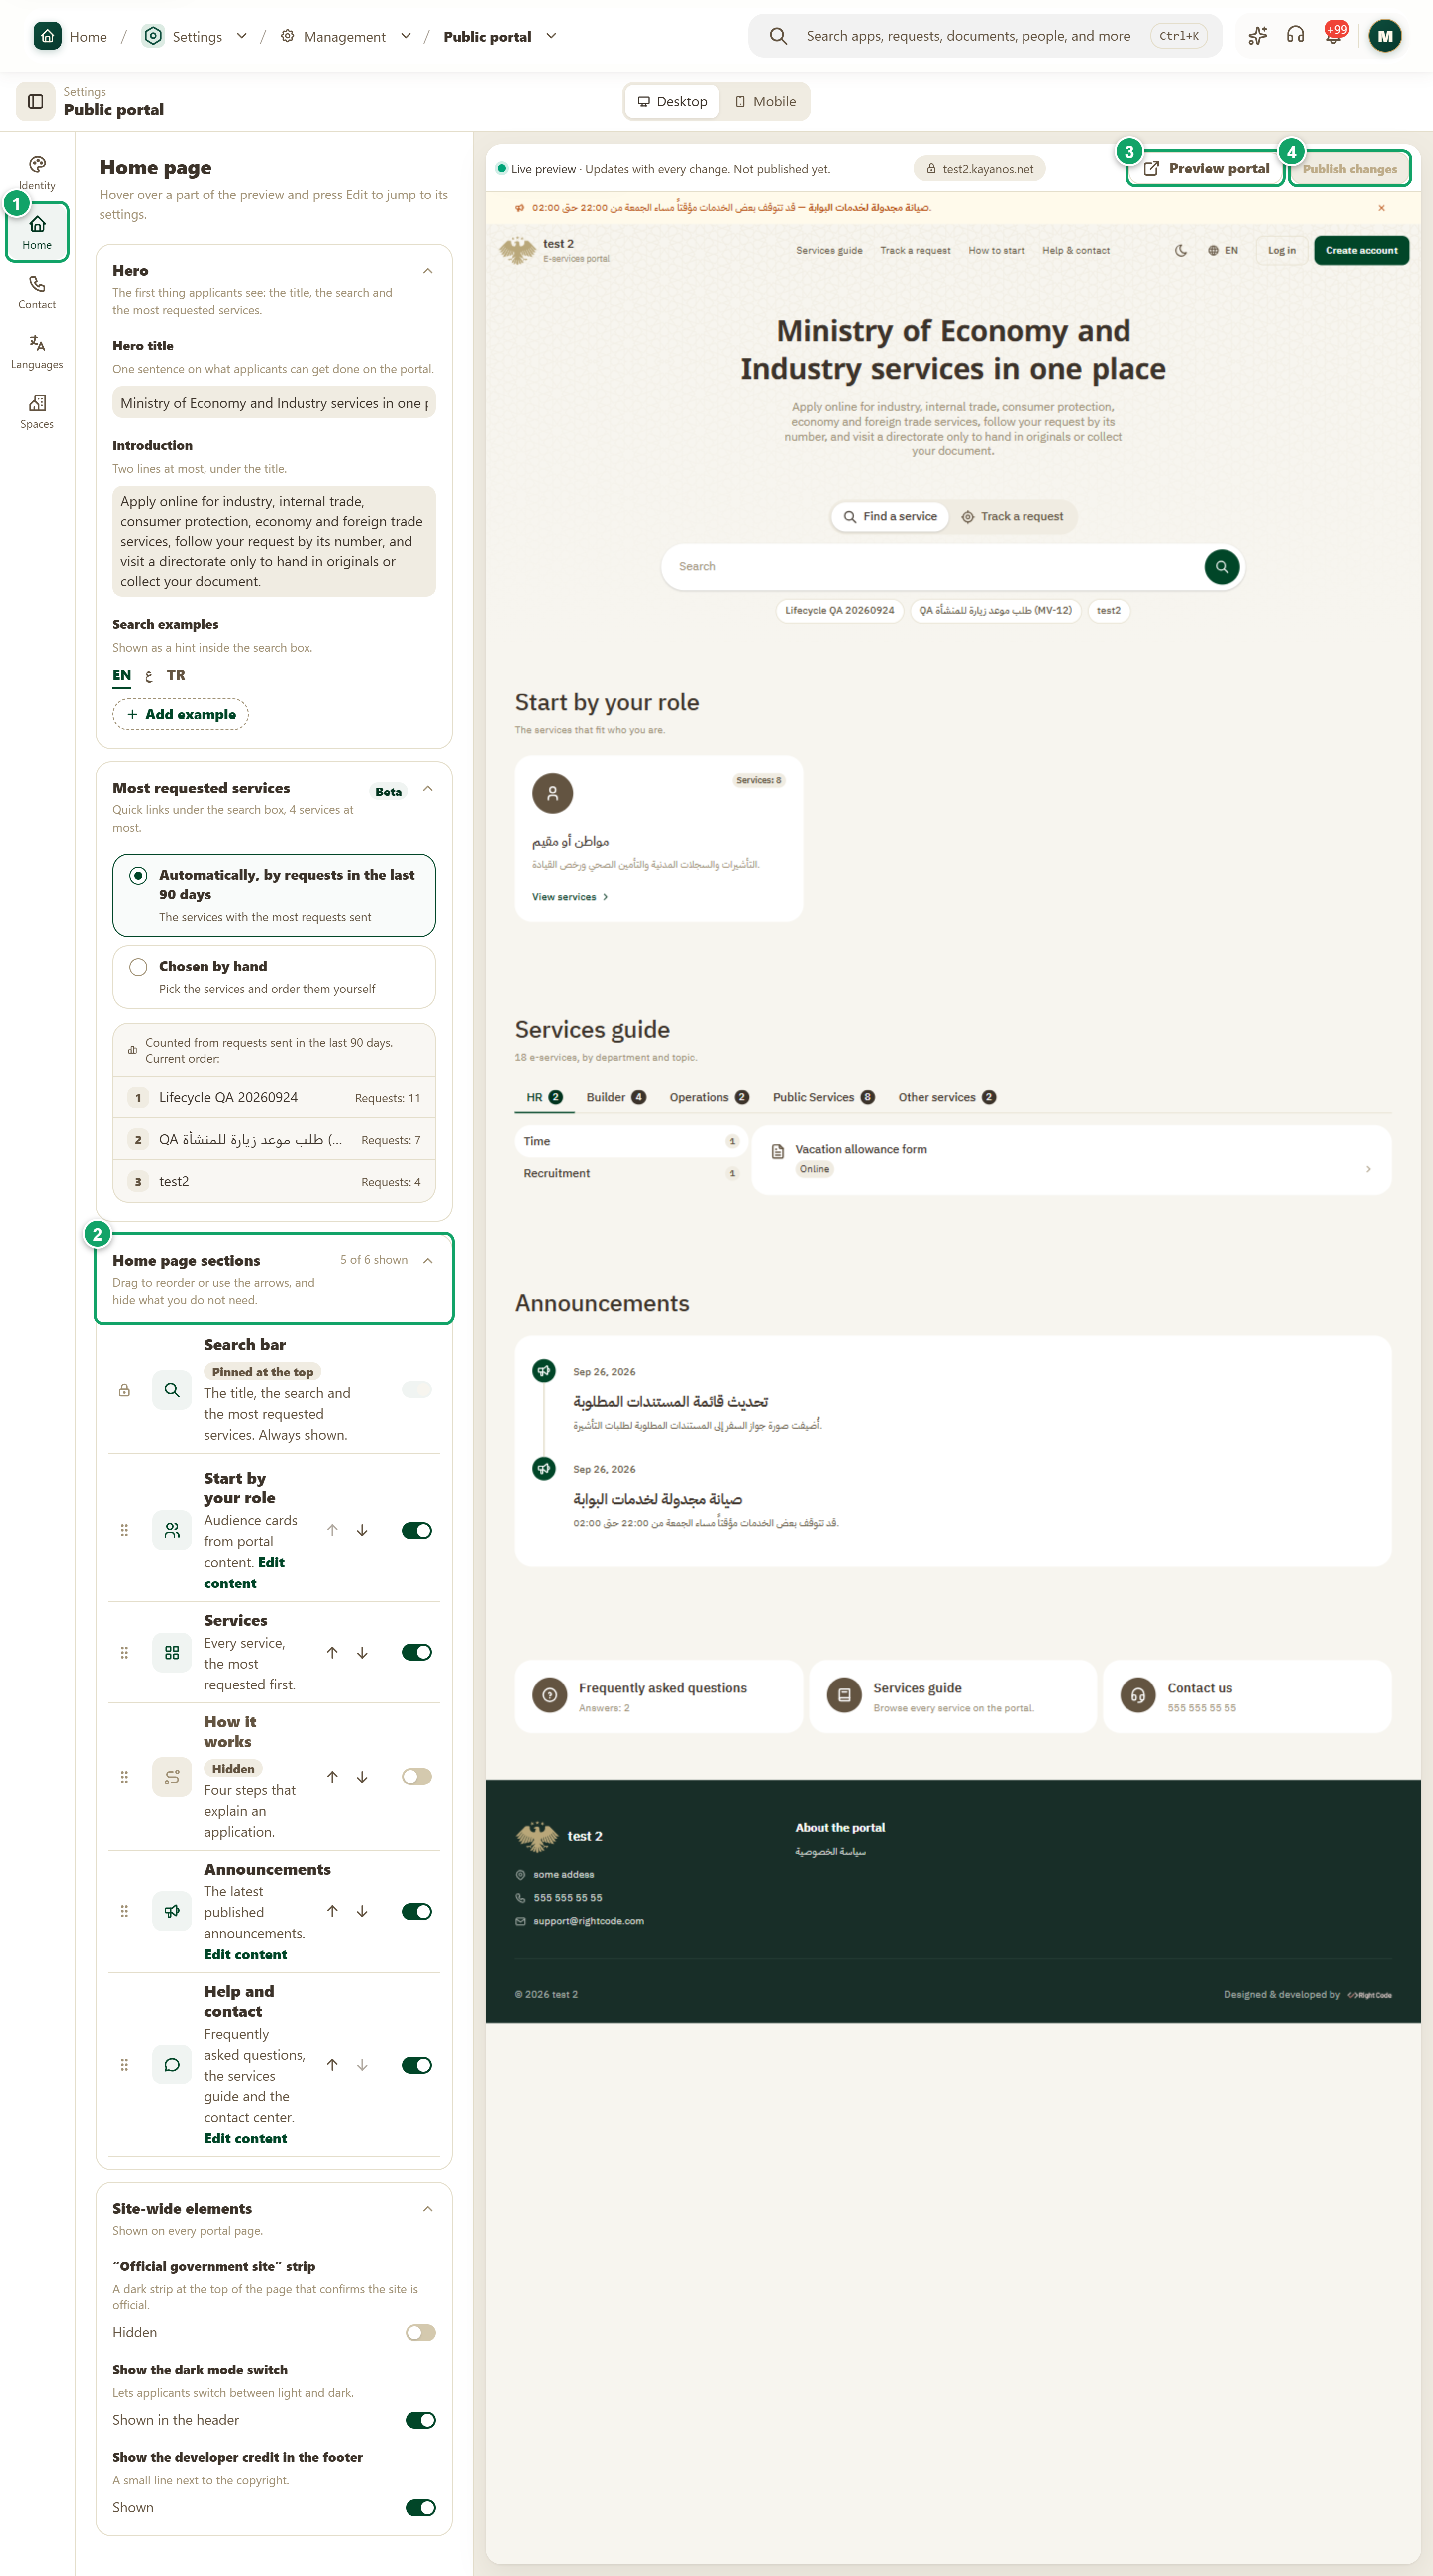
\includegraphics[width=0.95\linewidth,height=0.72\textheight,keepaspectratio]{figures/screens/ch08-public-portal-home-en.png}
\caption{The Home tab and the live preview}
\label{fig:settings-public-portal-home}
\shotnote{The image shows the settings panel beside a live preview of the portal, so you see each change before publishing it. The content shown is test data. ① “Home”. ② “Home page sections”: reorder the sections and hide what you do not need; the search bar stays pinned at the top. ③ “Preview portal”: opens the portal in a new window. ④ “Publish changes”: stays disabled until you edit something.}
\end{figure}

\begin{figure}[H]
\centering
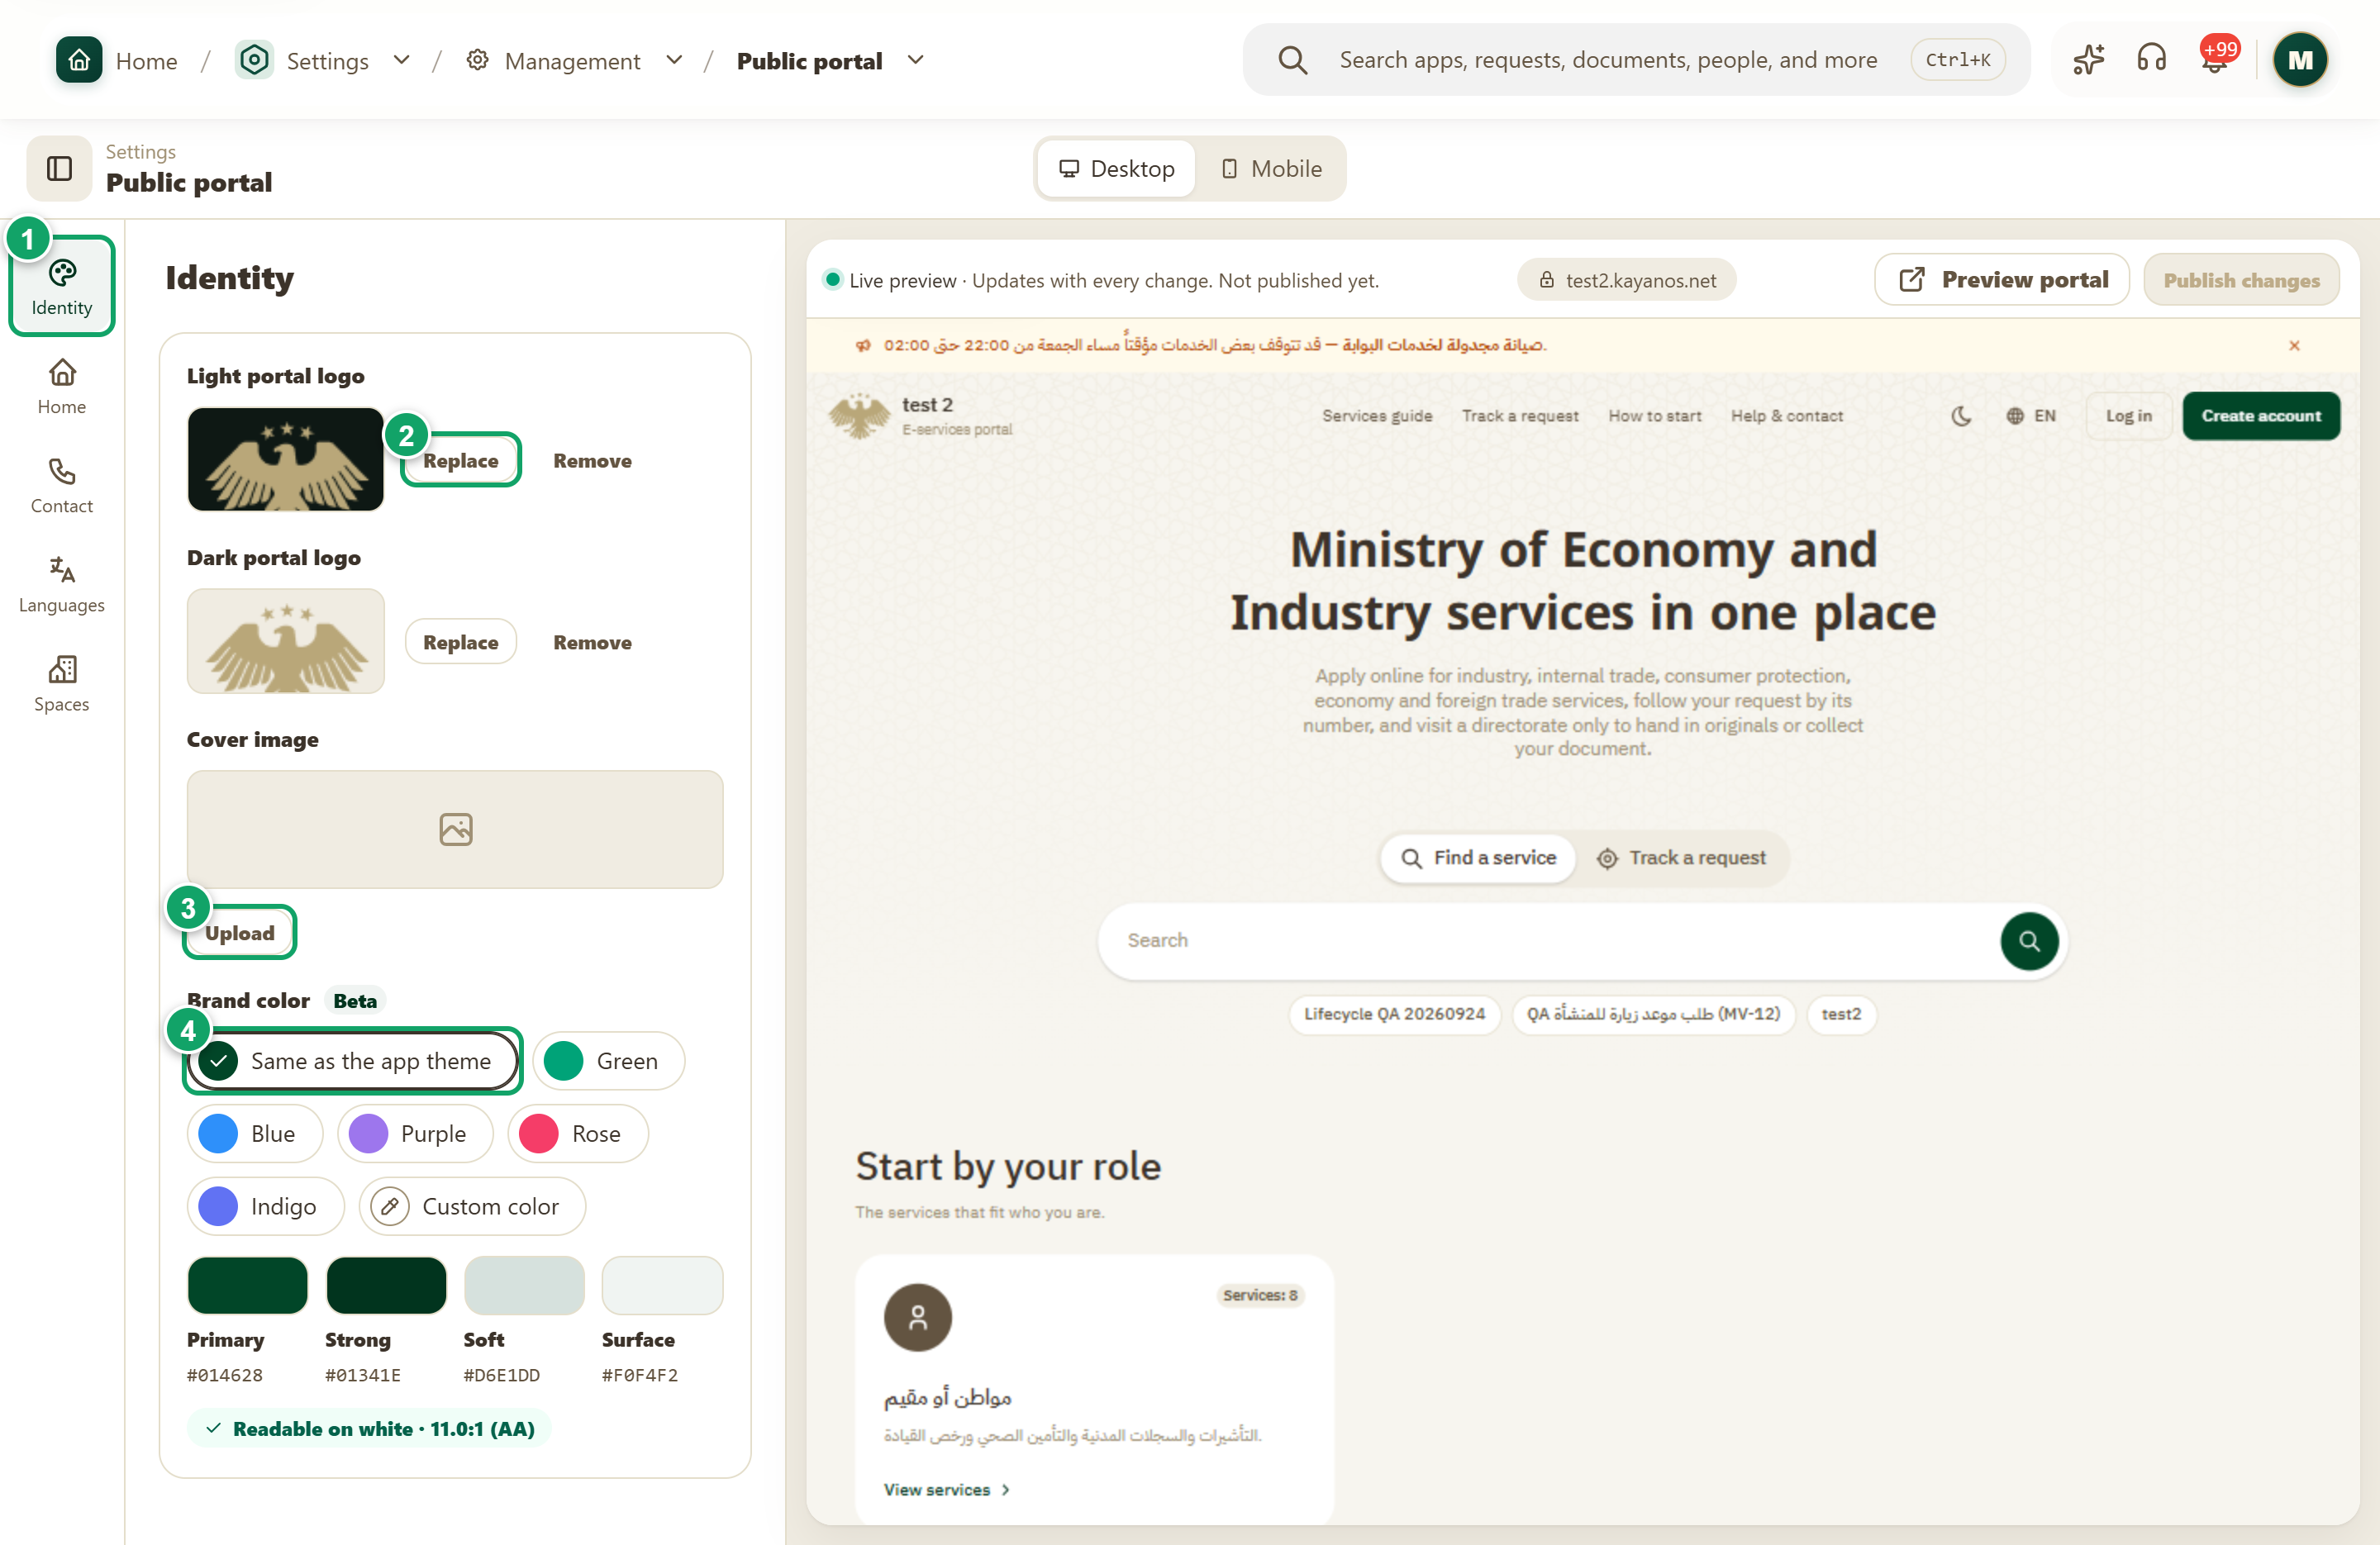
\includegraphics[width=0.95\linewidth,height=0.72\textheight,keepaspectratio]{figures/screens/ch08-public-portal-identity-en.png}
\caption{The Identity tab}
\label{fig:settings-public-portal-identity}
\shotnote{This tab sets the images and color that make the portal recognizably yours. The page checks the chosen color and shows whether text stays readable on white. ① “Identity”. ② “Replace”: changes the light logo, which appears on dark backgrounds. ③ “Upload”: adds the cover image. ④ “Same as the app theme”: makes the portal follow the app’s colors; you can pick another color beside it.}
\end{figure}

\begin{figure}[H]
\centering
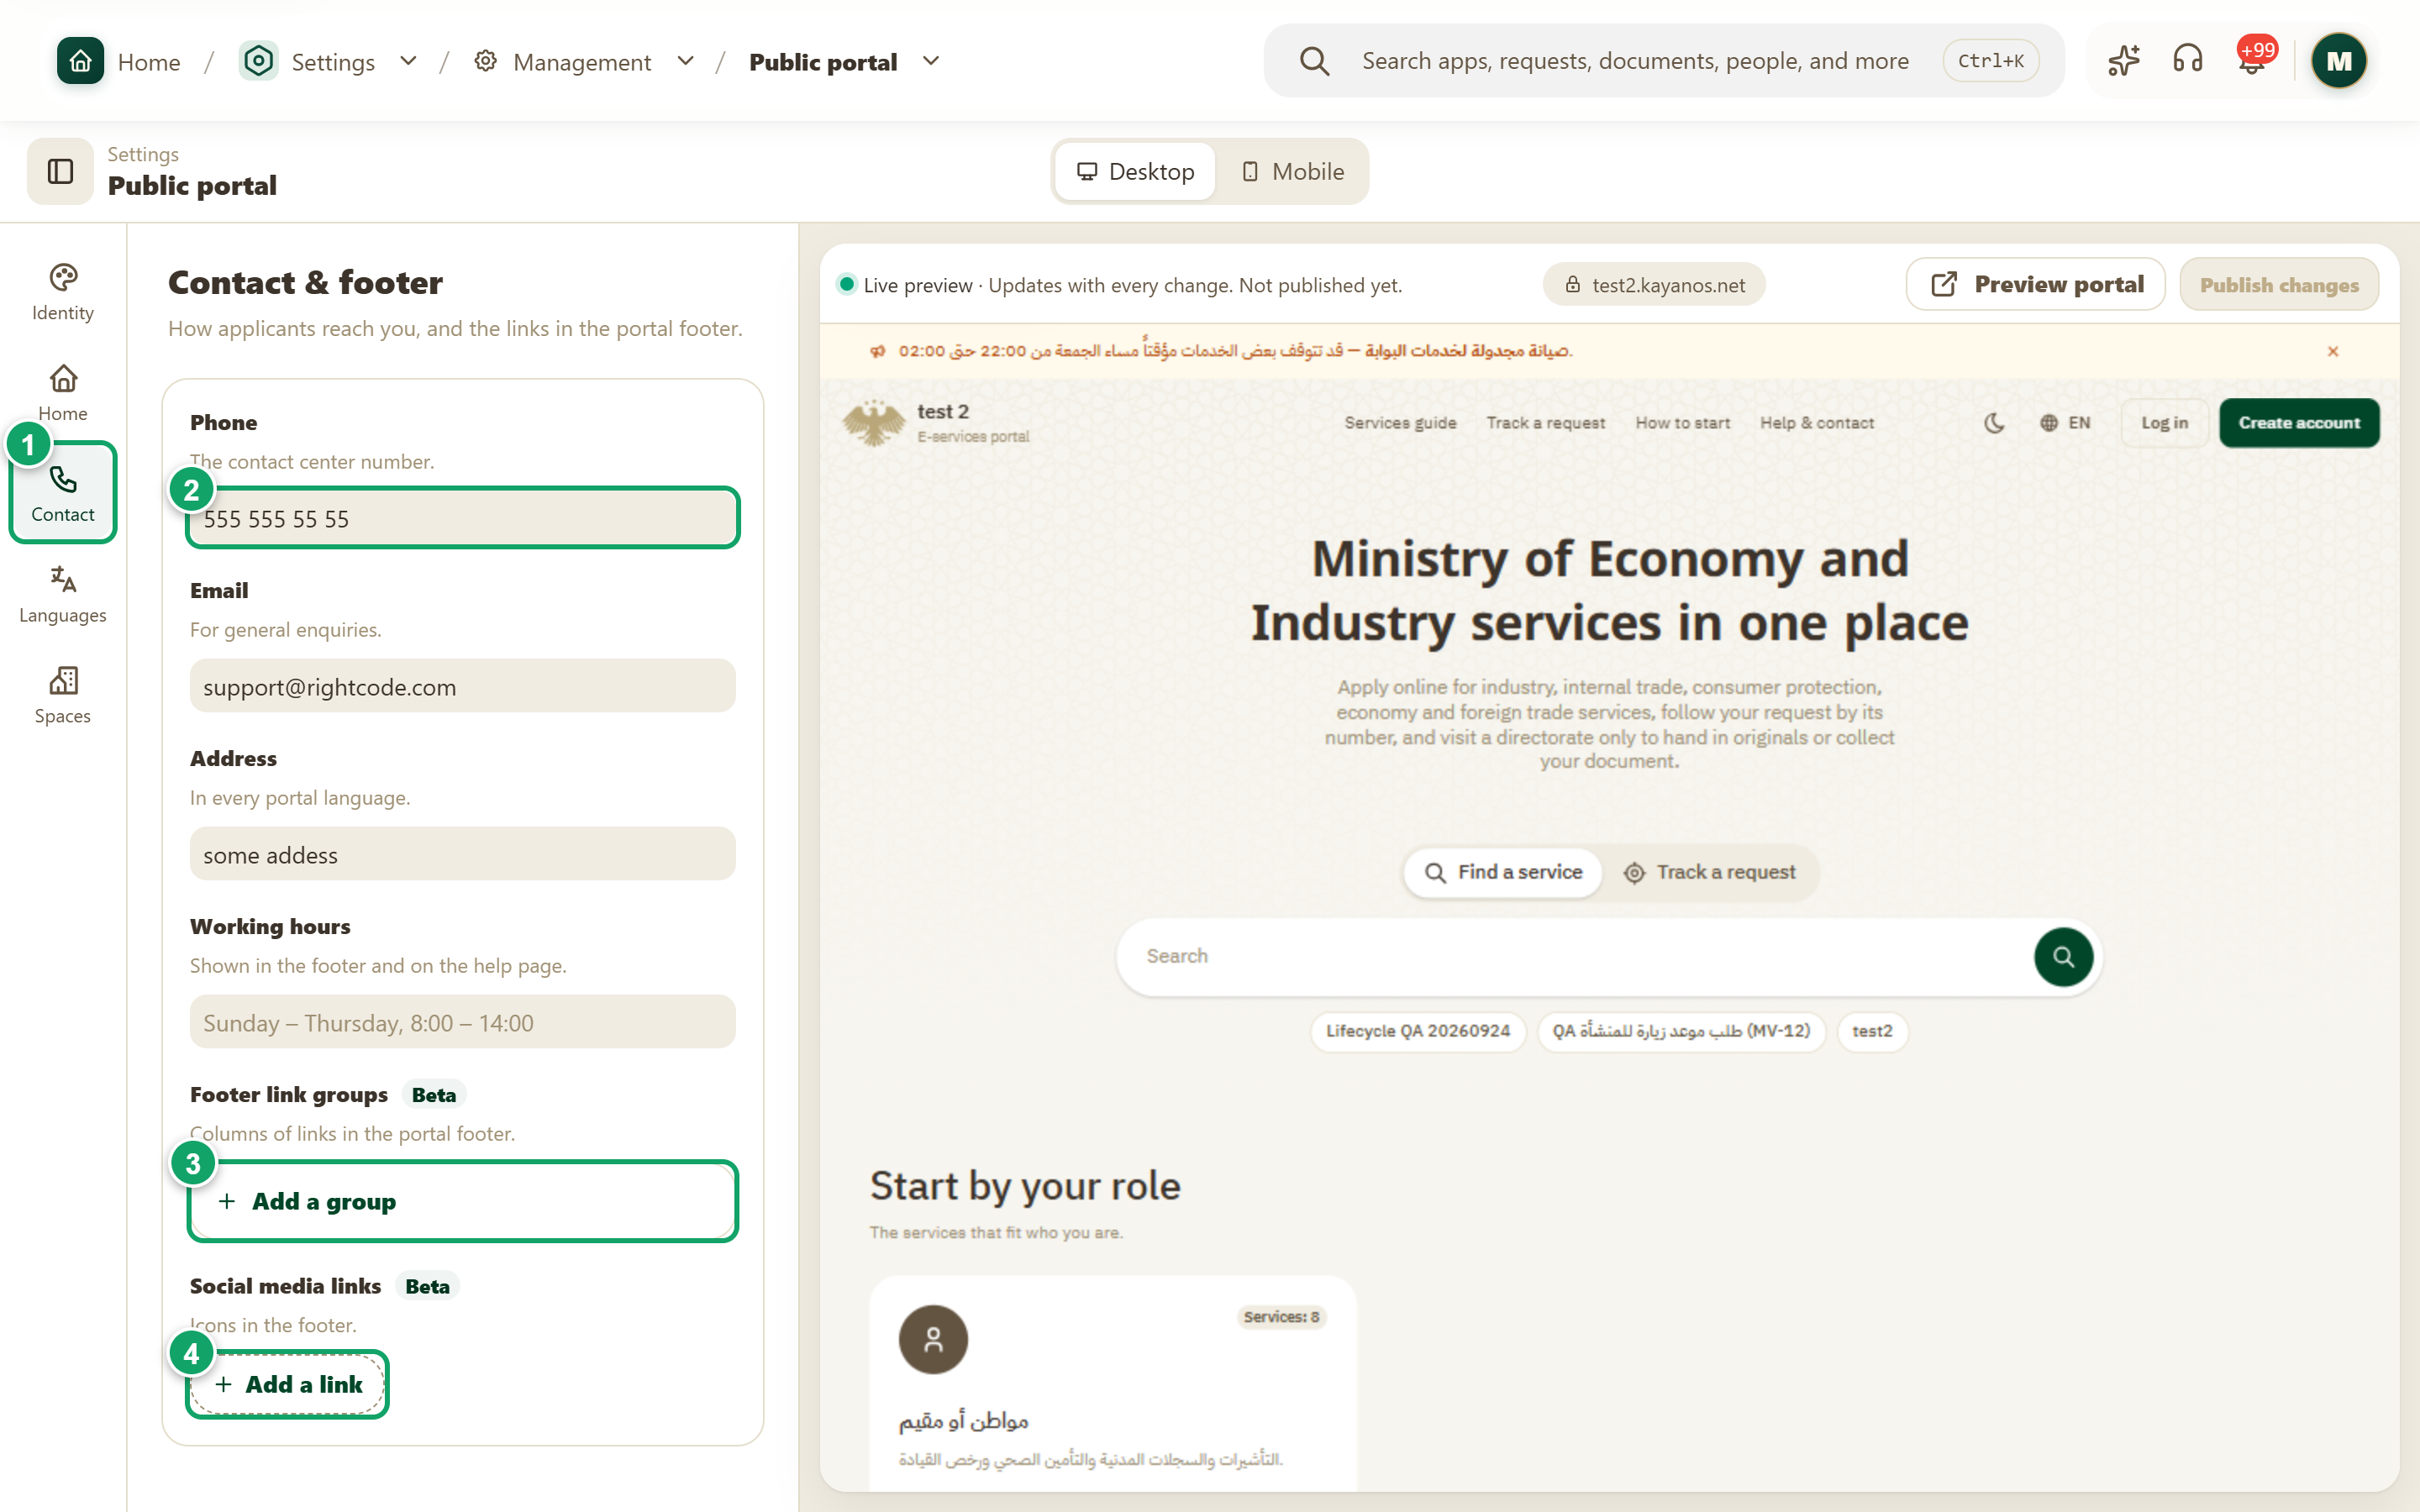
\includegraphics[width=0.95\linewidth,height=0.72\textheight,keepaspectratio]{figures/screens/ch08-public-portal-contact-en.png}
\caption{The Contact tab}
\label{fig:settings-public-portal-contact}
\shotnote{This tab holds what an applicant needs to reach you, and most of it appears in the portal footer, the fixed area at the bottom of every page. Publishing refuses an incomplete link: each link needs a name and a valid address. ① “Contact”. ② The “Phone” field: the contact center number. ③ “Add a group”: adds a column of links to the footer. ④ “Add a link”: adds a link to a social media account.}
\end{figure}

\begin{figure}[H]
\centering
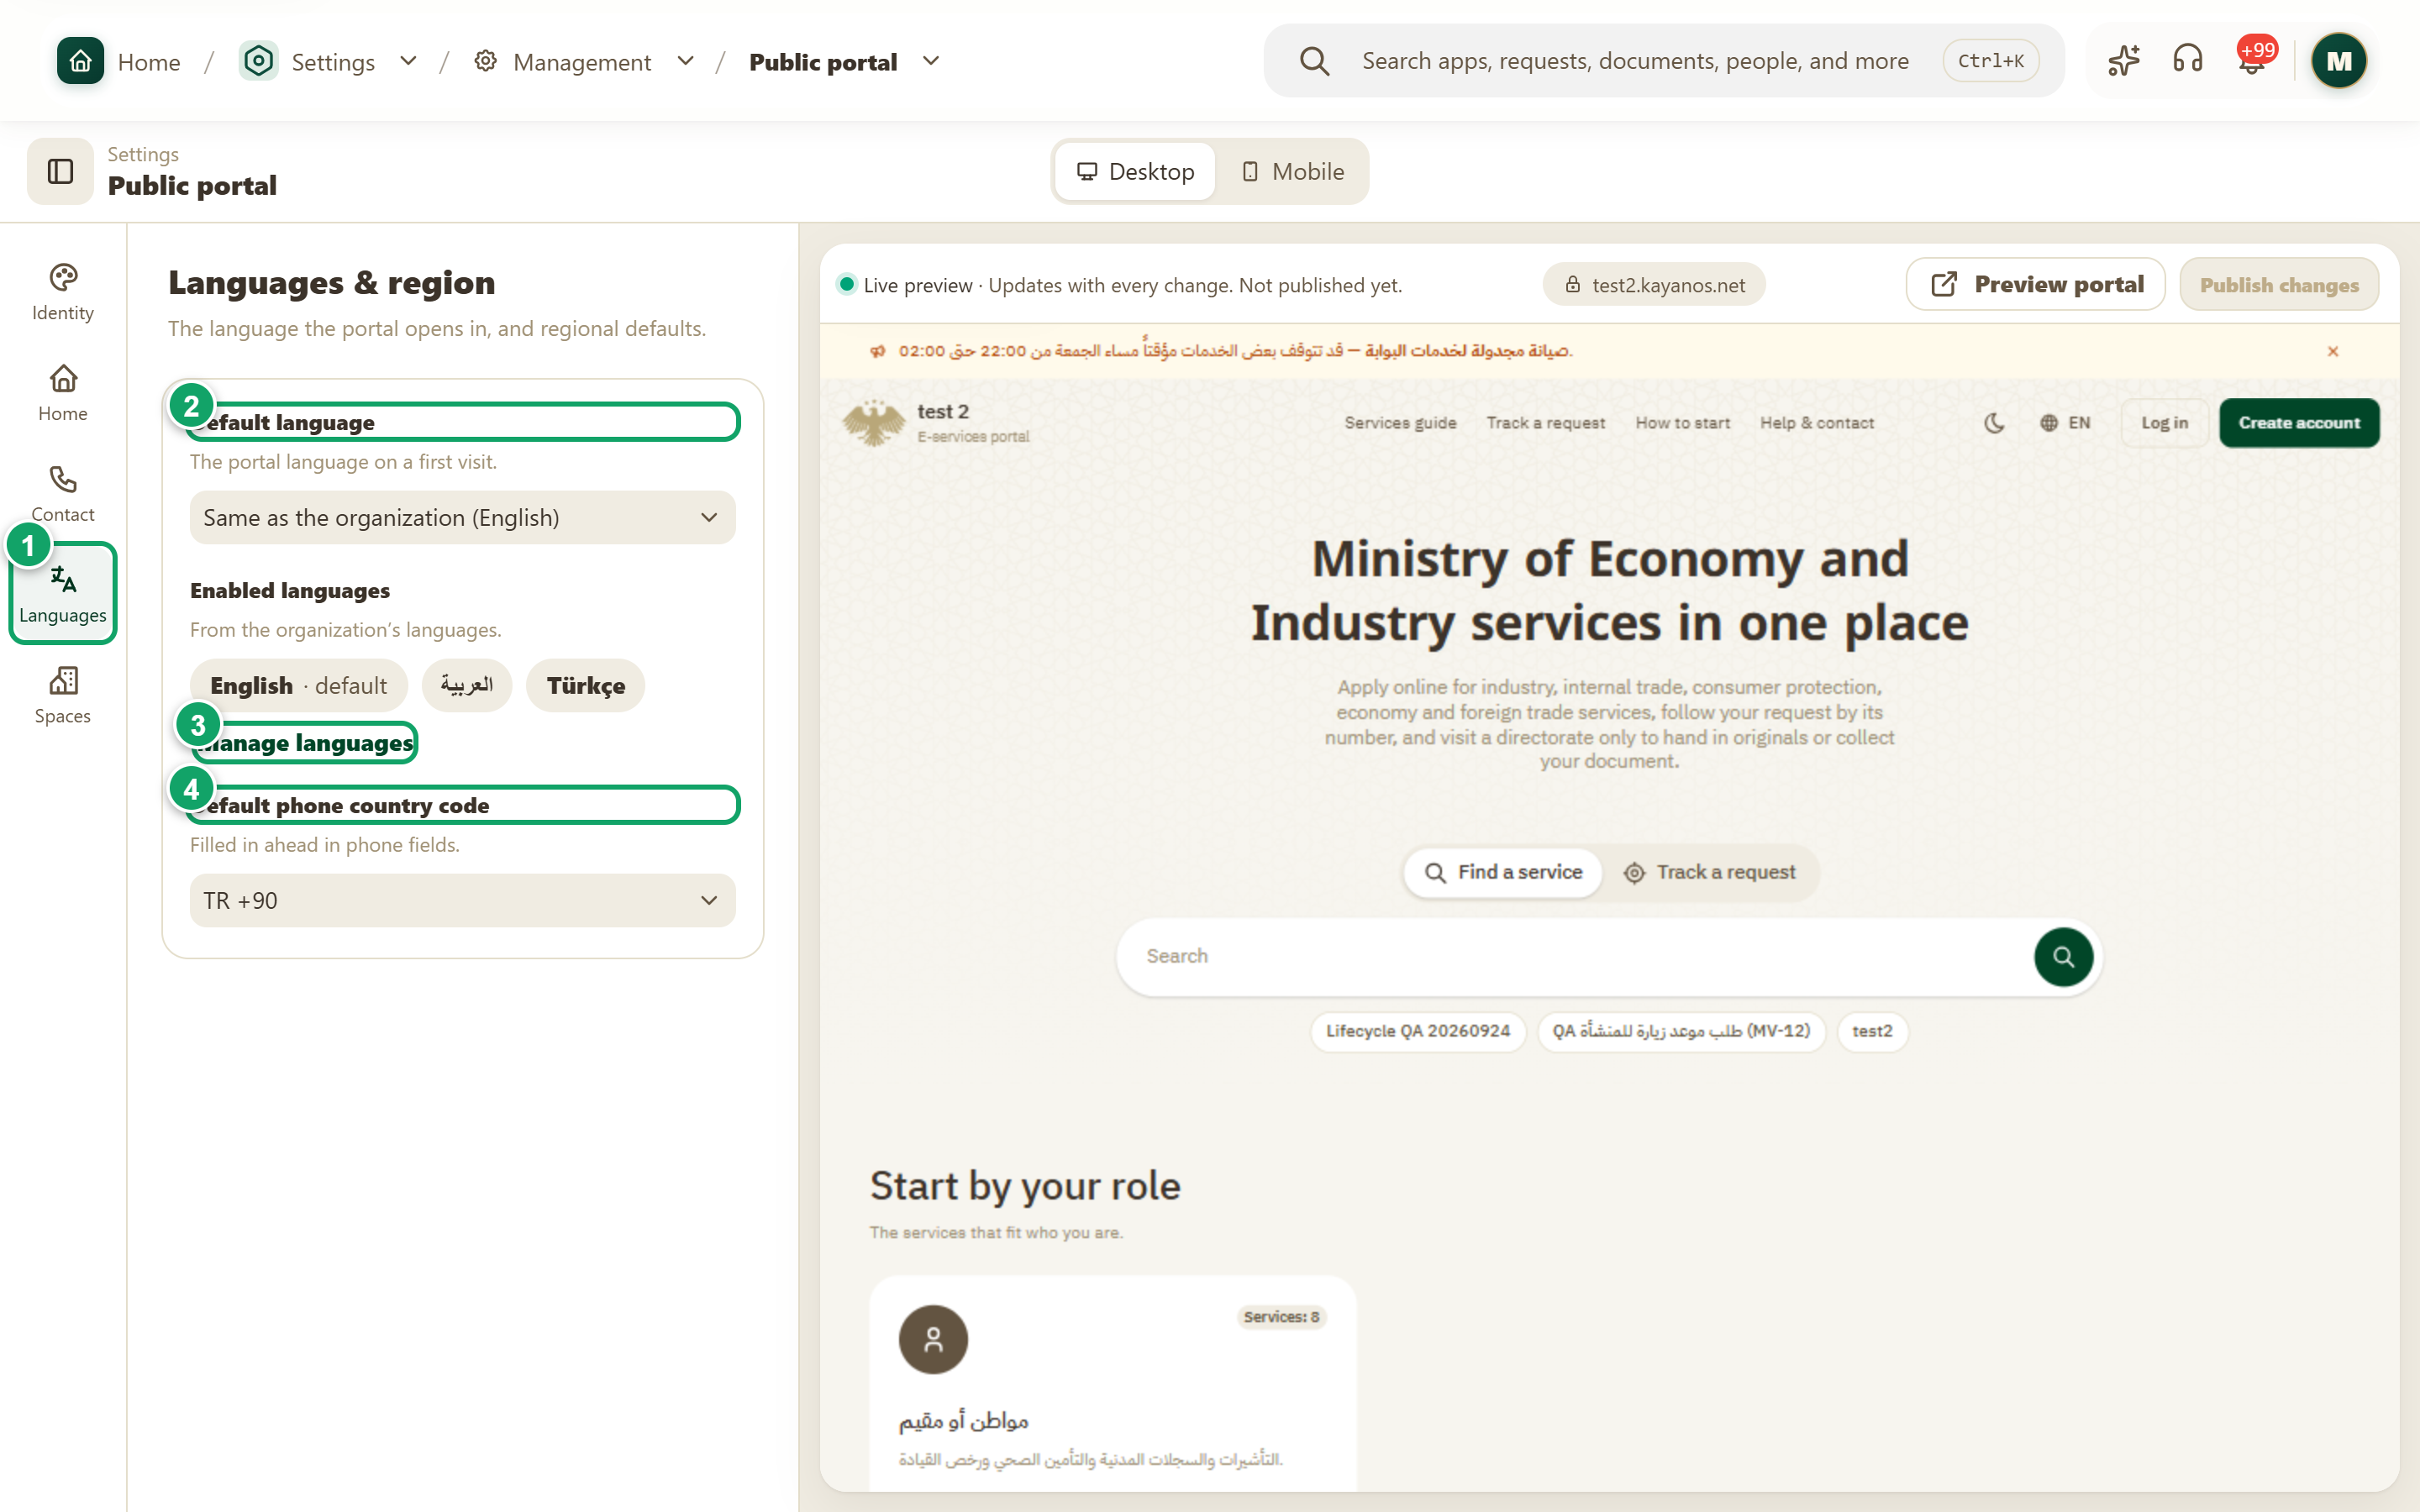
\includegraphics[width=0.95\linewidth,height=0.72\textheight,keepaspectratio]{figures/screens/ch08-public-portal-languages-en.png}
\caption{The Languages tab}
\label{fig:settings-public-portal-languages}
\shotnote{This tab sets the language a first-time visitor sees; the list of languages itself comes from the organization’s languages and is not edited here. ① “Languages”. ② “Default language”. ③ “Manage languages”: takes you to the organization’s languages page. ④ “Default phone country code”: filled in ahead in phone fields.}
\end{figure}

\begin{figure}[H]
\centering
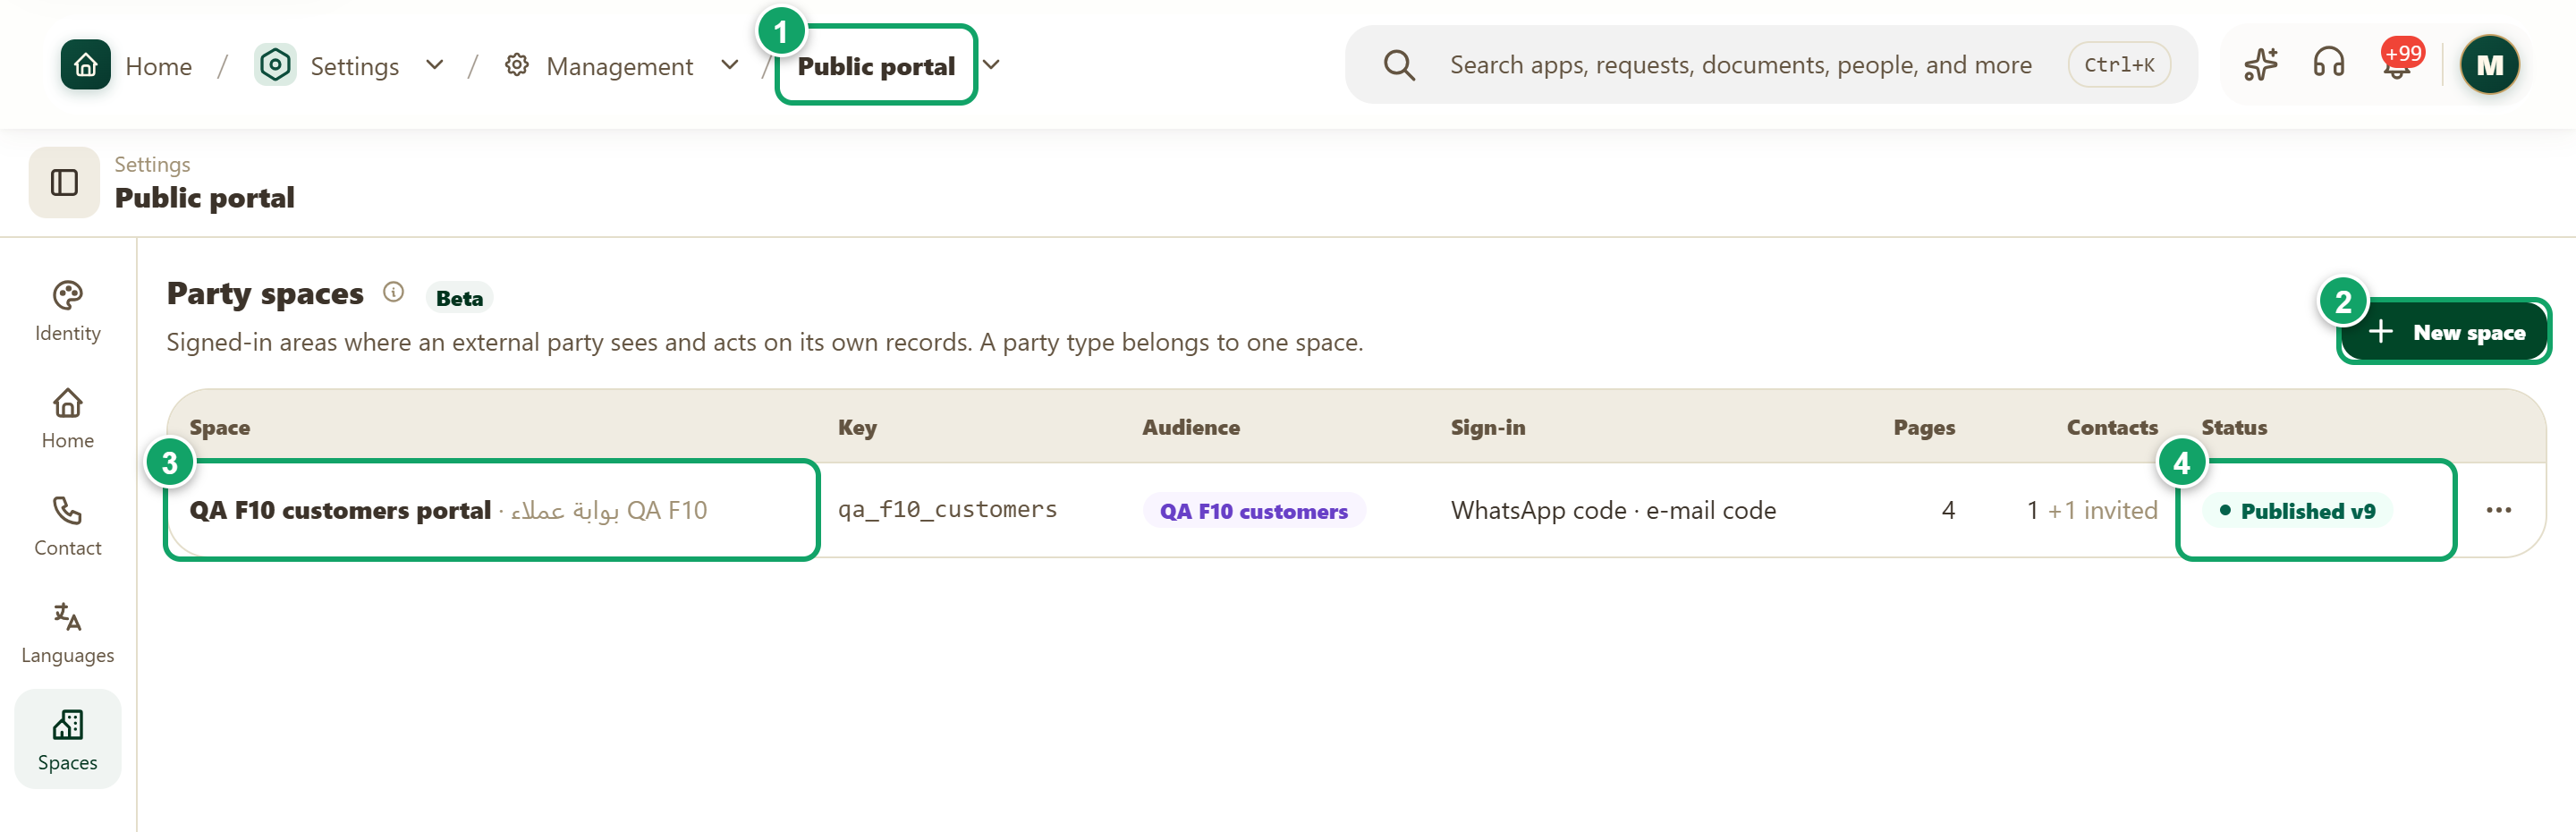
\includegraphics[width=0.95\linewidth,height=0.72\textheight,keepaspectratio]{figures/screens/ch08-public-portal-spaces-en.png}
\caption{The Spaces tab}
\label{fig:settings-public-portal-spaces}
\shotnote{A space is an area where an outside party, such as a customer or supplier, signs in to see and work on its own records. Each space has its own publishing, so “Publish changes” does not cover it. The row shown is a test space. ① “Spaces”. ② “New space”. ③ The space’s name. ④ The space’s status and published version.}
\end{figure}

\begin{table}[H]
\centering
\caption{What do you record on the public portal?}
\label{tab:settings-public-portal-fields}
\begin{tabularx}{\linewidth}{R{4.2cm} Y}
\rcHeaderRow
\thh{Tab} & \thh{What do you set?}\\
“Identity” & “Light portal logo”, “Dark portal logo” and “Cover image”, each up to 5 MB, then “Brand color”.\\
“Home” & “Hero”: “Hero title”, “Introduction” and “Search examples”. “Most requested services”: automatic from the last 90 days of requests or “Chosen by hand”, four at most. “Home page sections”. “Site-wide elements”: the “Official government site” strip, the dark mode switch and the developer credit in the footer.\\
“Contact” & “Phone”, “Email”, “Address” and “Working hours”, then “Footer link groups”, up to four groups of eight links each, and “Social media links”, up to eight.\\
“Languages” & “Default language”, which follows the organization’s language unless you choose another, and “Default phone country code”. “Enabled languages” is shown for reference.\\
“Spaces” & The “Party spaces” list, where you create a space and edit its sections: “Audience”, “Sign-in”, “Contacts \& roles”, “Pages”, “Record types”, “Actions”, “Confirmations”, “Notifications”, “Branding” and “Security”.\\
\end{tabularx}
\end{table}

\begin{enumerate}
\item Open “Settings”, then “Public portal”.
\item Choose the tab you want from the side column and edit its values.
\item Check the result in the preview, switching between “Desktop” and “Mobile” to see both screens.
\item Hover over a part of the preview and press “Edit” to jump straight to its settings.
\item Press “Publish changes”. Publishing covers the edits on the first four tabs together.
\end{enumerate}

\textbf{Check:} “Saved” appears beside the publish button. Press “Preview portal” and confirm your edit shows on the portal. If the page moves you to the “Contact” tab with an error, complete or remove the incomplete footer link and publish again.

\clearpage
\section{Portal content}
\label{sec:settings-feature-portal-content}

Where “Public portal” sets the overall look, this page holds what applicants read: audience cards, long pages such as a privacy policy, frequently asked questions and announcements. An audience is a group of services brought together by who the applicant is, such as an investor or a training center.

Use this page whenever you add or update text without changing the portal’s settings. The organization owner and holders of the Administrator role open it. Its items do not need the publish button: each one saves on its own, and the show switch in the table takes effect as soon as you press it.

\begin{rcnote}[Example: Horizon]
Horizon’s system administrator adds an announcement that the Aleppo branch closes for a day, and at ② chooses to show it as a strip on every page. He sets its dates at ③, then confirms the switch at ④ is on before saving.
\end{rcnote}
\begin{figure}[H]
\centering
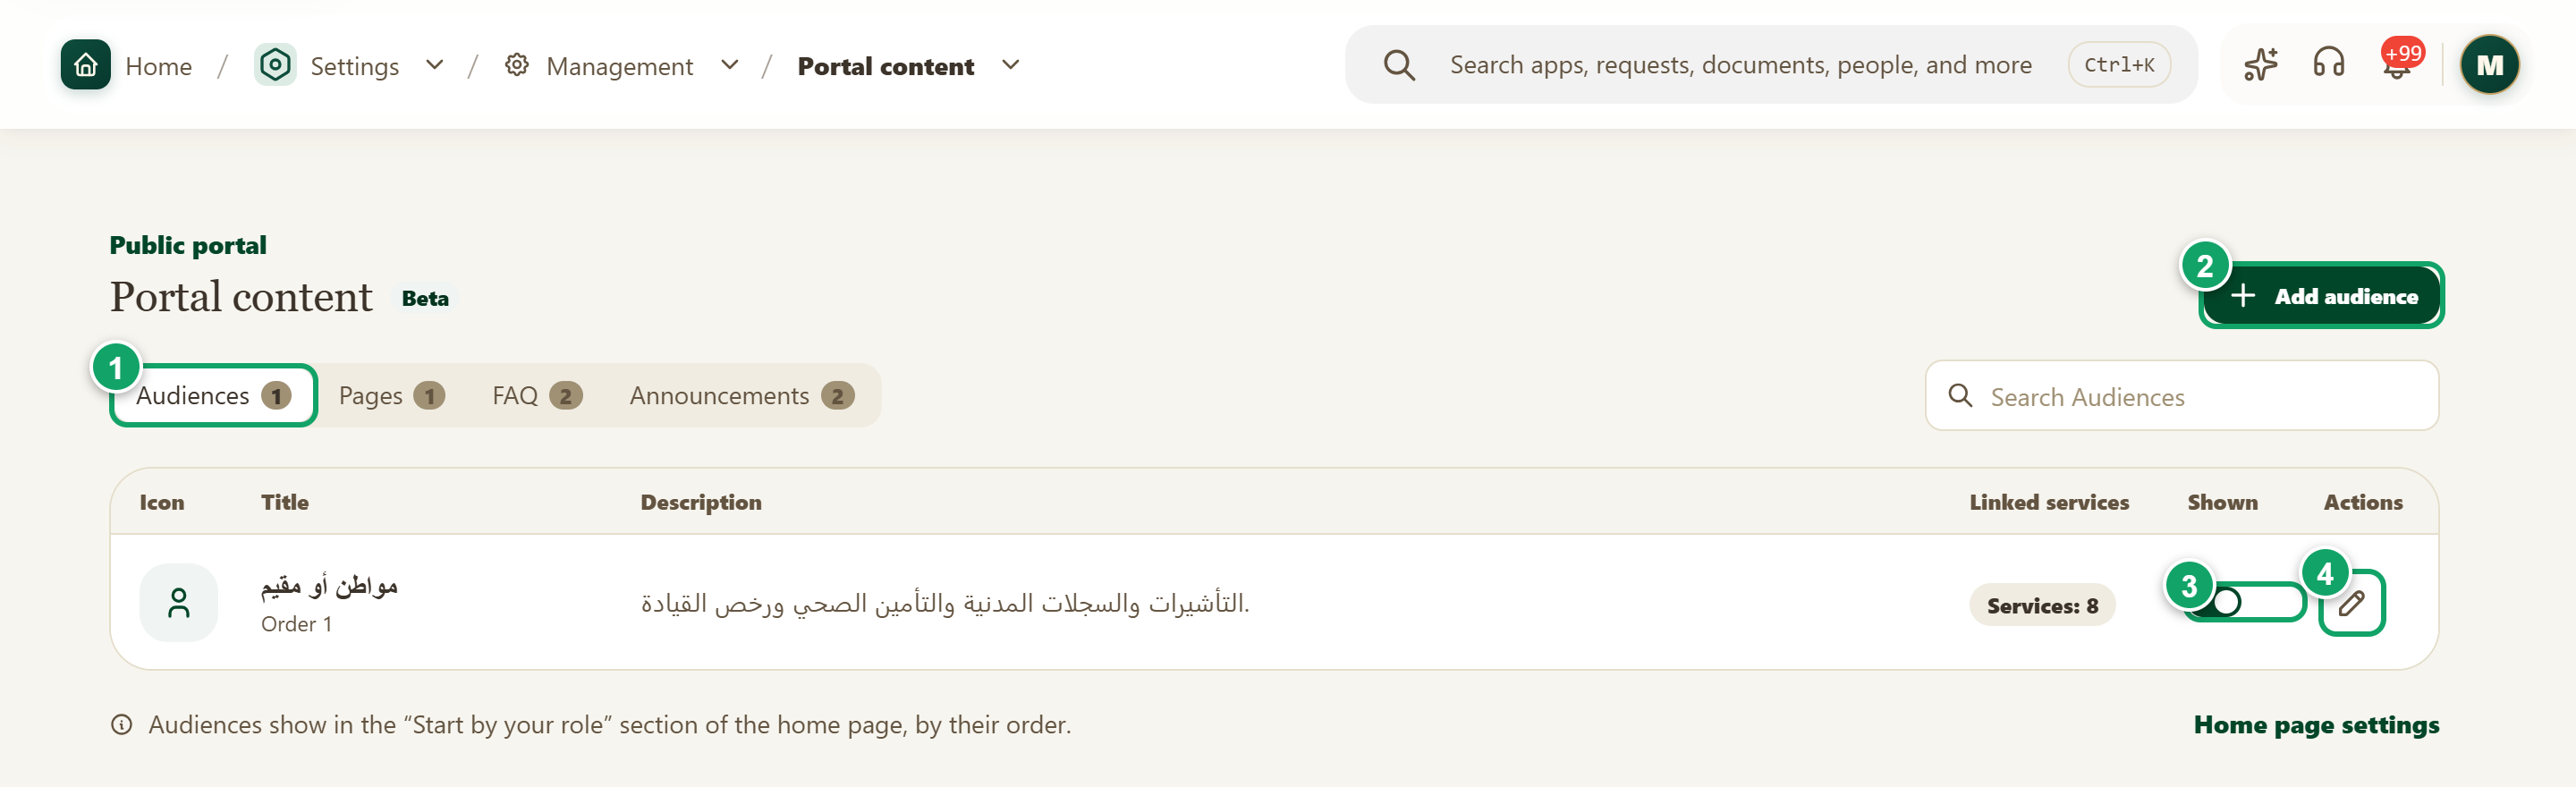
\includegraphics[width=0.95\linewidth,height=0.72\textheight,keepaspectratio]{figures/screens/ch08-portal-content-audience-en.png}
\caption{Audiences}
\label{fig:settings-portal-content-audience}
\shotnote{Audiences appear as cards in the “Start by your role” section of the home page, so applicants reach their services without knowing their names. The row shown is test data. ① “Audiences”. ② “Add audience”. ③ The “Shown” switch: hides or shows the card at once. ④ The edit button.}
\end{figure}

\begin{figure}[H]
\centering
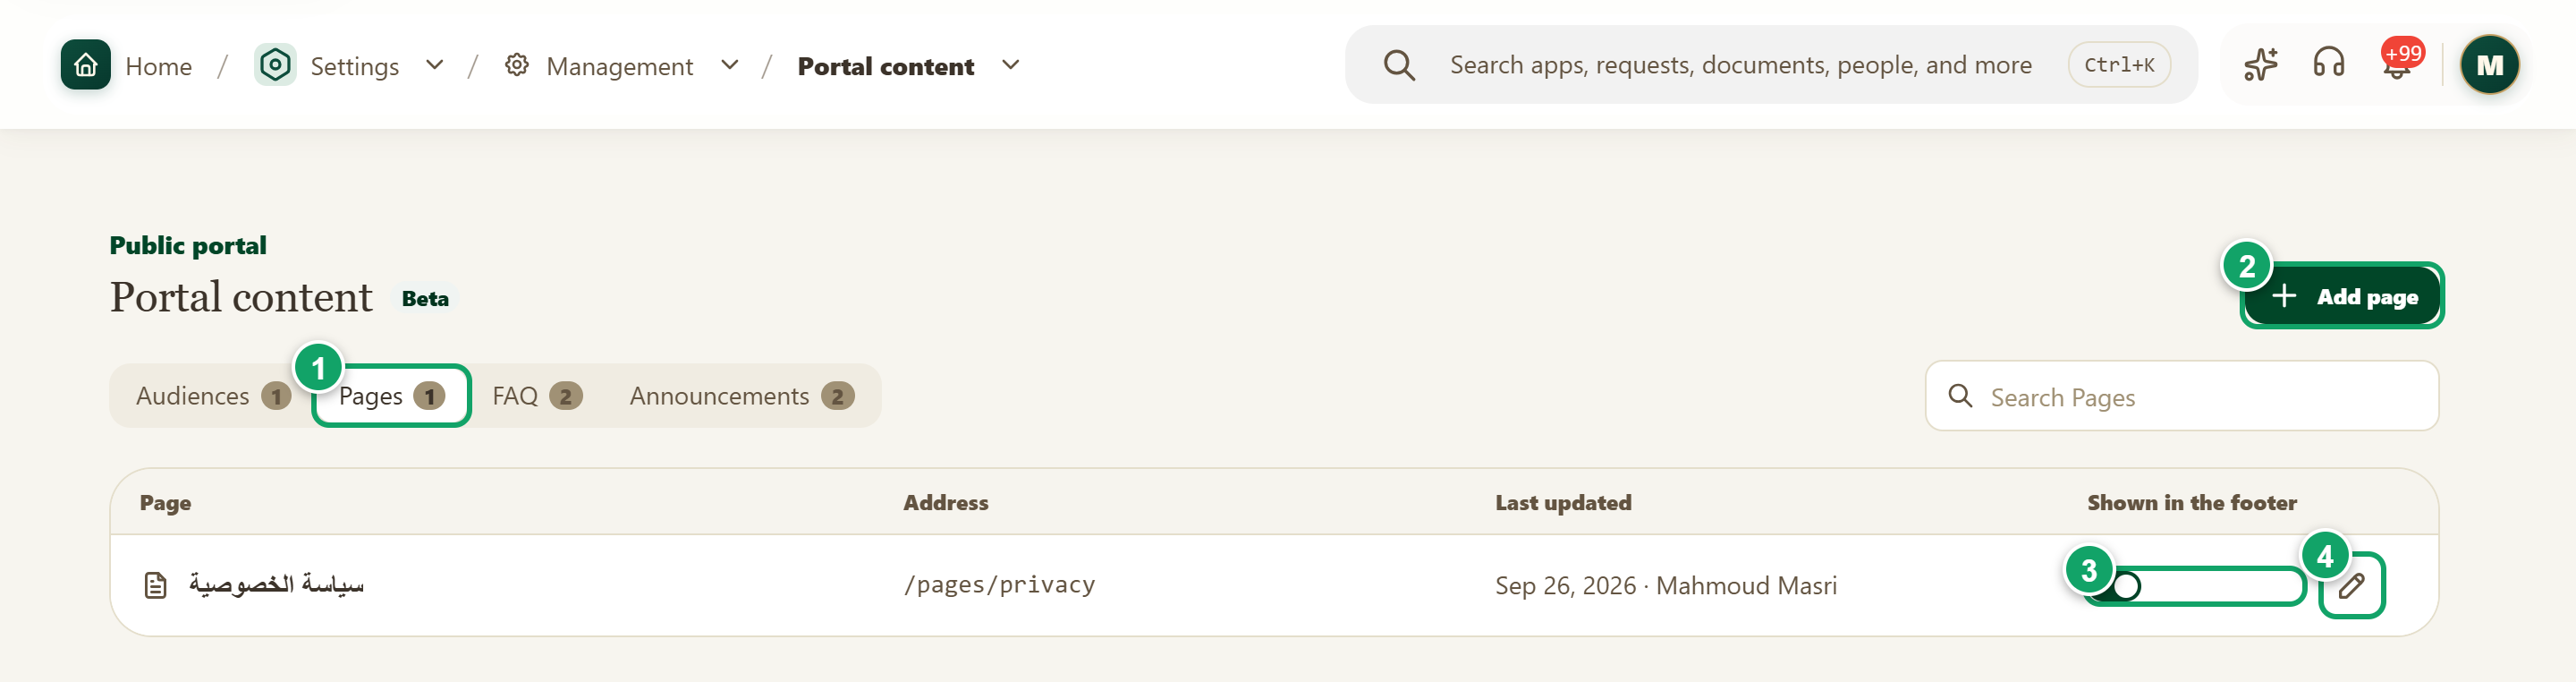
\includegraphics[width=0.95\linewidth,height=0.72\textheight,keepaspectratio]{figures/screens/ch08-portal-content-page-en.png}
\caption{Pages}
\label{fig:settings-portal-content-page}
\shotnote{Pages hold long texts, and each has a fixed address shown in the table. The switch controls only whether it appears in the footer, so it stays available to anyone with its address. ① “Pages”. ② “Add page”. ③ The “Shown in the footer” switch. ④ The edit button.}
\end{figure}

\begin{figure}[H]
\centering
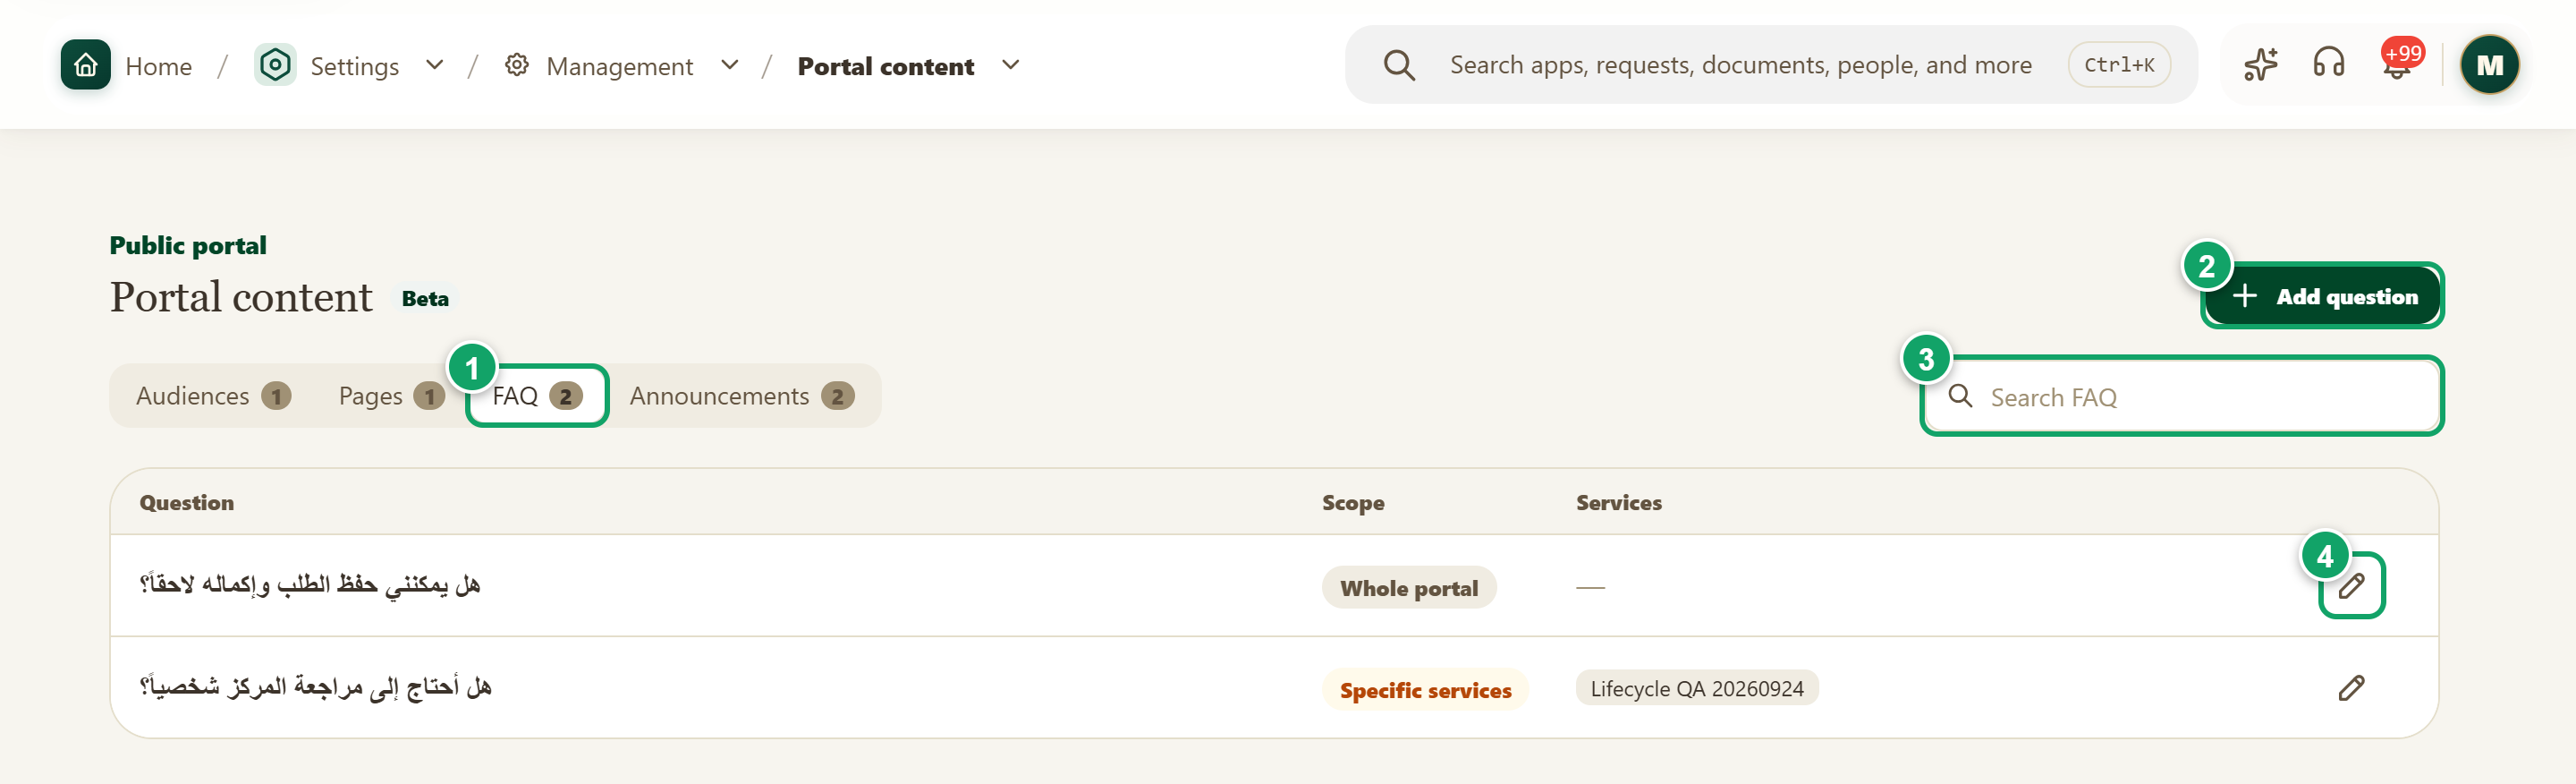
\includegraphics[width=0.95\linewidth,height=0.72\textheight,keepaspectratio]{figures/screens/ch08-portal-content-faq-en.png}
\caption{Frequently asked questions}
\label{fig:settings-portal-content-faq}
\shotnote{“Scope” decides where a question appears: on the help page alone, or also on an app’s services or on specific services. A question linked to a service therefore helps the people actually applying for it. ① “FAQ”. ② “Add question”. ③ The search field. ④ The edit button.}
\end{figure}

\begin{figure}[H]
\centering
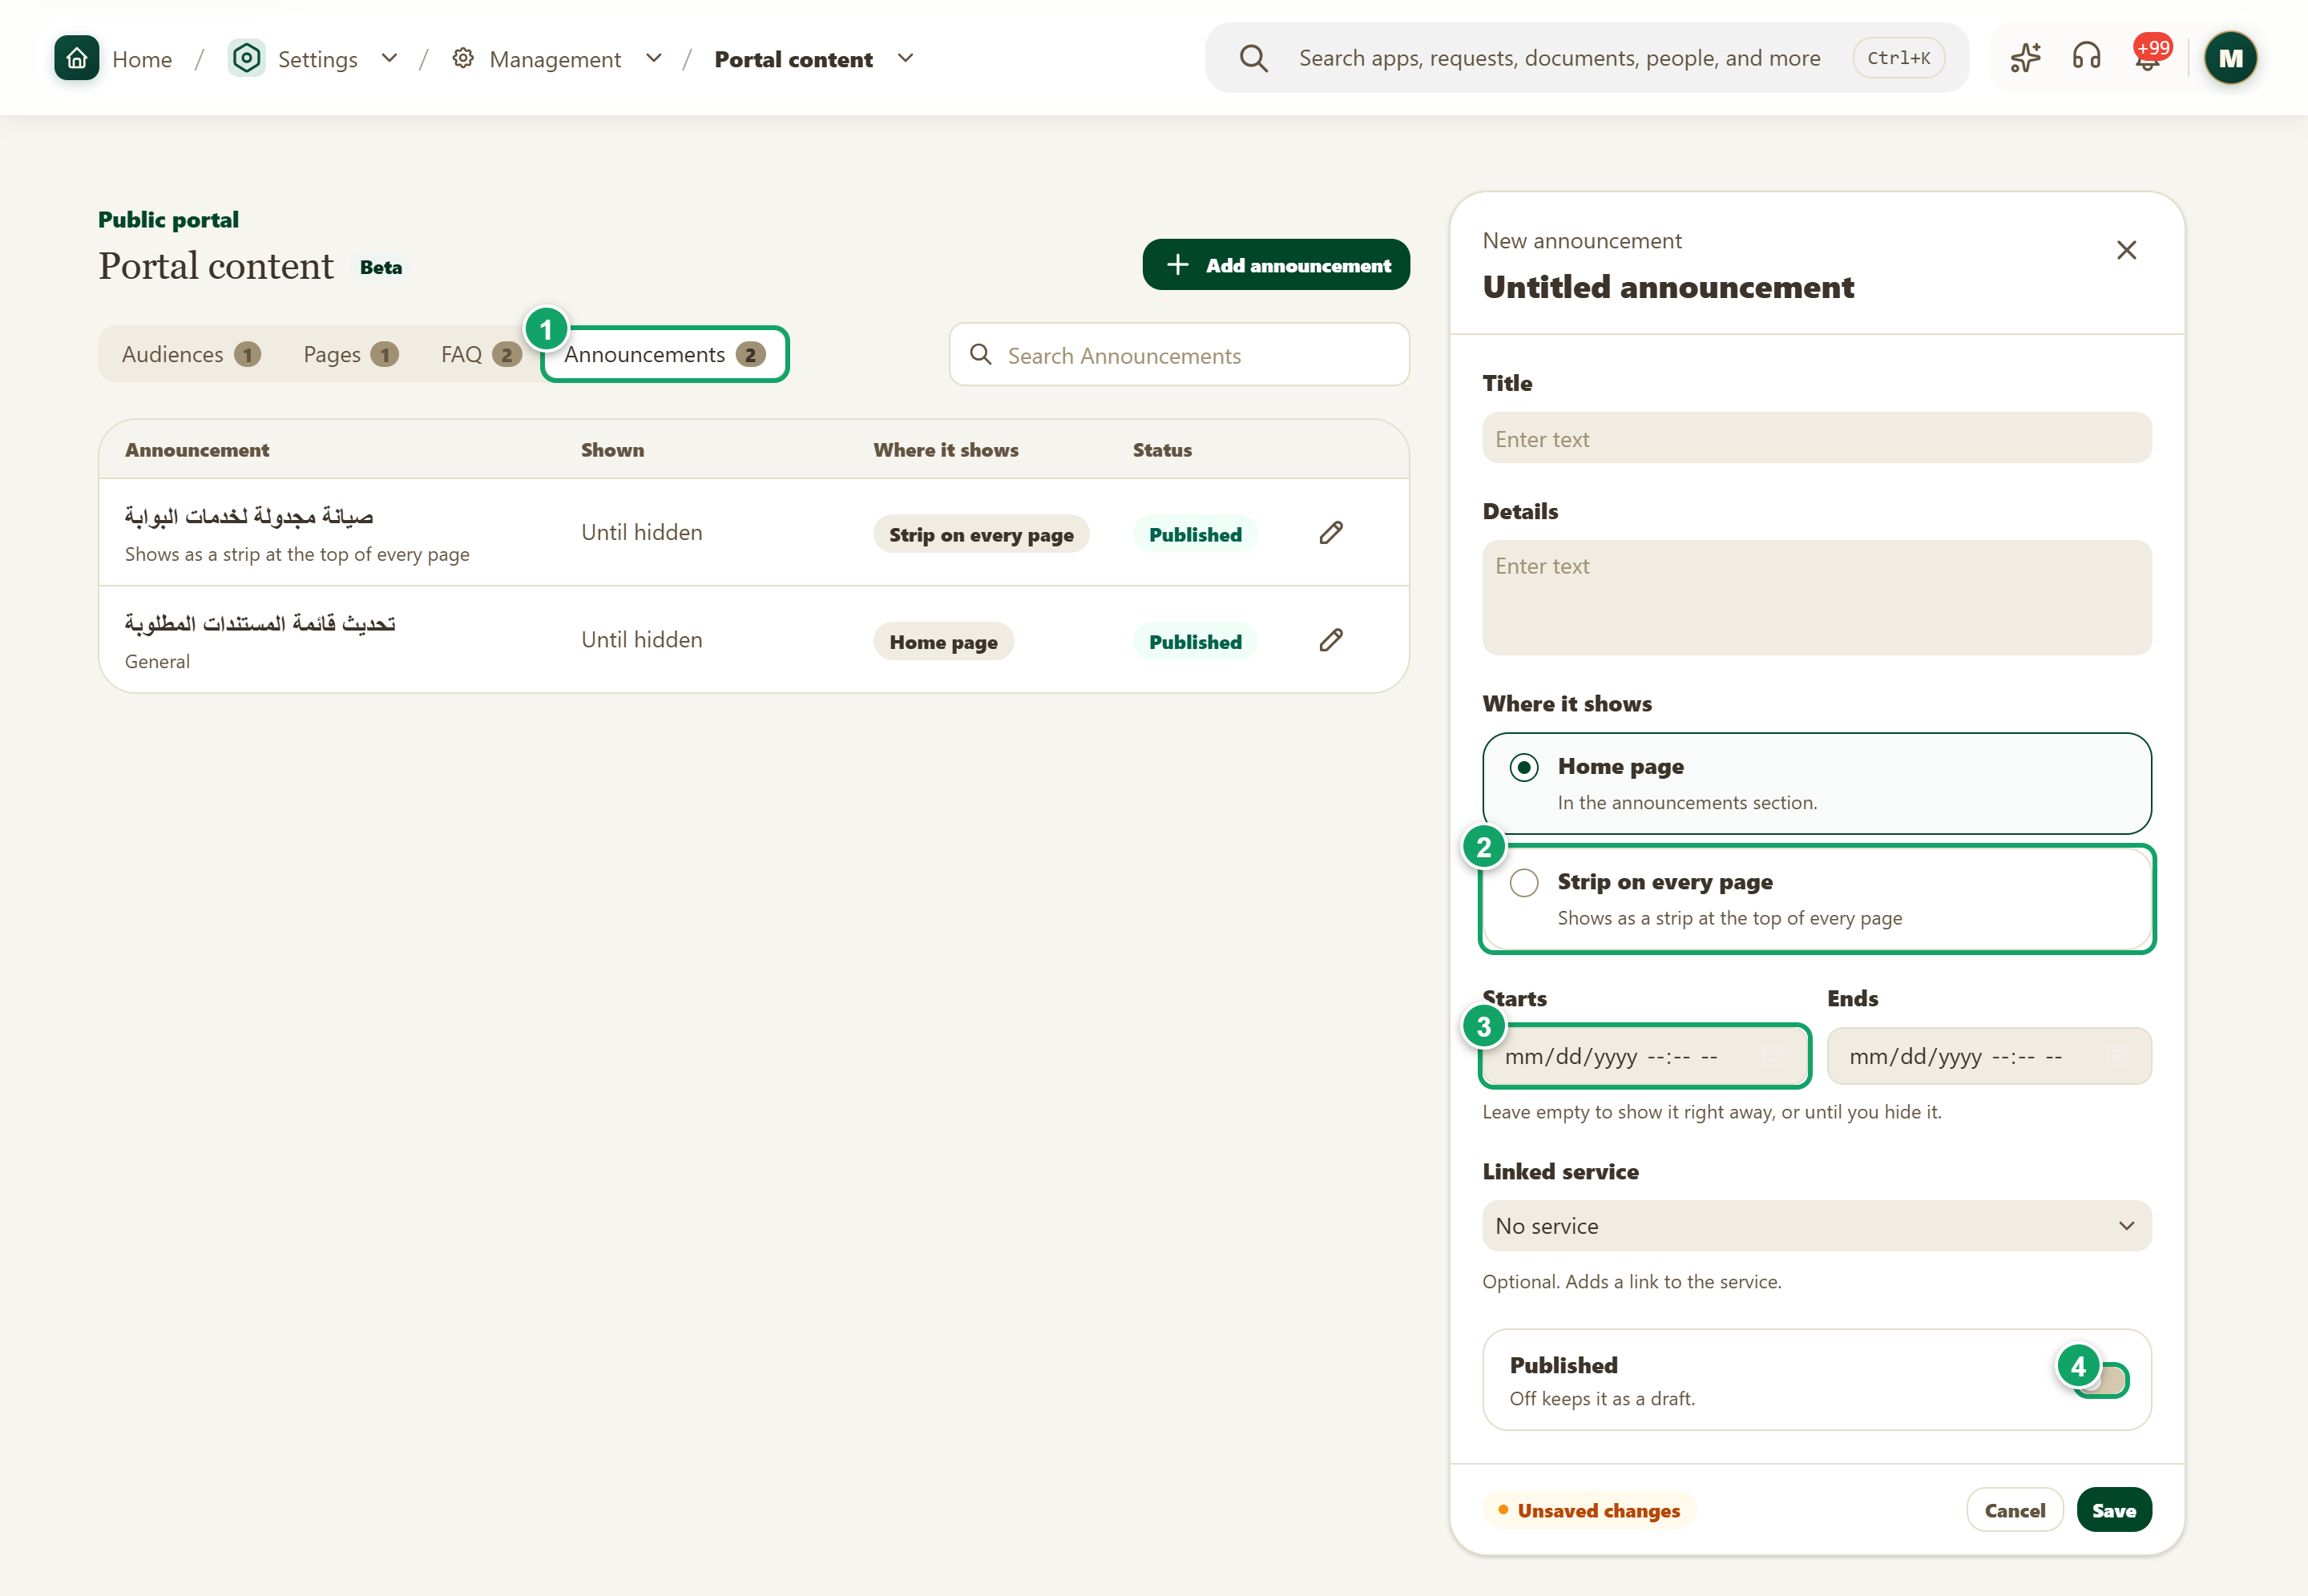
\includegraphics[width=0.95\linewidth,height=0.72\textheight,keepaspectratio]{figures/screens/ch08-portal-content-announcement-en.png}
\caption{The new announcement form}
\label{fig:settings-portal-content-announcement}
\shotnote{The form opens beside the table without leaving the page; the one shown is empty and was not saved. A new announcement stays a draft until you turn on the publish switch. ① “Announcements”. ② “Strip on every page”: the alternative to showing it in the home page’s announcements section. ③ The “Starts” field: leave it empty to show the announcement at once, and leave “Ends” empty to keep it until you hide it. ④ The “Published” switch.}
\end{figure}

\begin{table}[H]
\centering
\caption{What do you record in portal content?}
\label{tab:settings-portal-content-fields}
\begin{tabularx}{\linewidth}{R{4.2cm} Y}
\rcHeaderRow
\thh{Tab} & \thh{What do you record?}\\
“Audiences” & “Title”, “Description” and “Icon”, then the services it shows from “Apps”, “Sections” and “More services”, and finally “Order”: the smaller number appears first.\\
“Pages” & “Title”, “Address” in lowercase Latin letters, numbers and hyphens, “Content” and “Shown in the footer”.\\
“FAQ” & “Question”, “Answer” and “Scope”: “Whole portal”, “App” or “Specific services”.\\
“Announcements” & “Title”, “Details”, “Where it shows”, “Starts”, “Ends”, “Linked service” and “Published”. The status reads “Published”, “Scheduled”, “Ended” or “Draft”.\\
\end{tabularx}
\end{table}

\begin{enumerate}
\item Open “Settings”, then “Portal content”.
\item Choose the content type from the tabs, then press the add button or the edit button on a row.
\item Fill in the form. Write text fields in every language you want applicants to read.
\item Press “Save”. If you edit and then close the form, the page asks before discarding your changes.
\item To delete an item, open it, press “Delete” and confirm; applicants will no longer see it.
\end{enumerate}

\textbf{Check:} The item appears in its table and the count beside the tab name goes up. Open the portal and confirm it shows in its place. If audiences or announcements do not appear, check whether their section is hidden in “Home page sections”.

\clearpage
\section{Applicant accounts}
\label{sec:settings-feature-applicant-profile}

An applicant creates one account to submit requests, so they do not repeat their details each time. This page decides what they fill in on their profile, when it is asked for, and how it is confirmed. Verification means confirming a value is correct, either with a code sent to their phone or email or through a staff member’s review.

Come back to this page before publishing services that need reliable details, such as a national ID number. The organization owner and holders of the Administrator role open it. “Company” holds the settings for applicants who represent companies.

\begin{rcnote}[Example: Horizon]
One Horizon service needs a reliable ID number, so the system administrator adds the field at ② and has staff verify it. He then creates a verification level at ⑤ that requires this field, so he can demand it on that service.
\end{rcnote}
\begin{figure}[H]
\centering
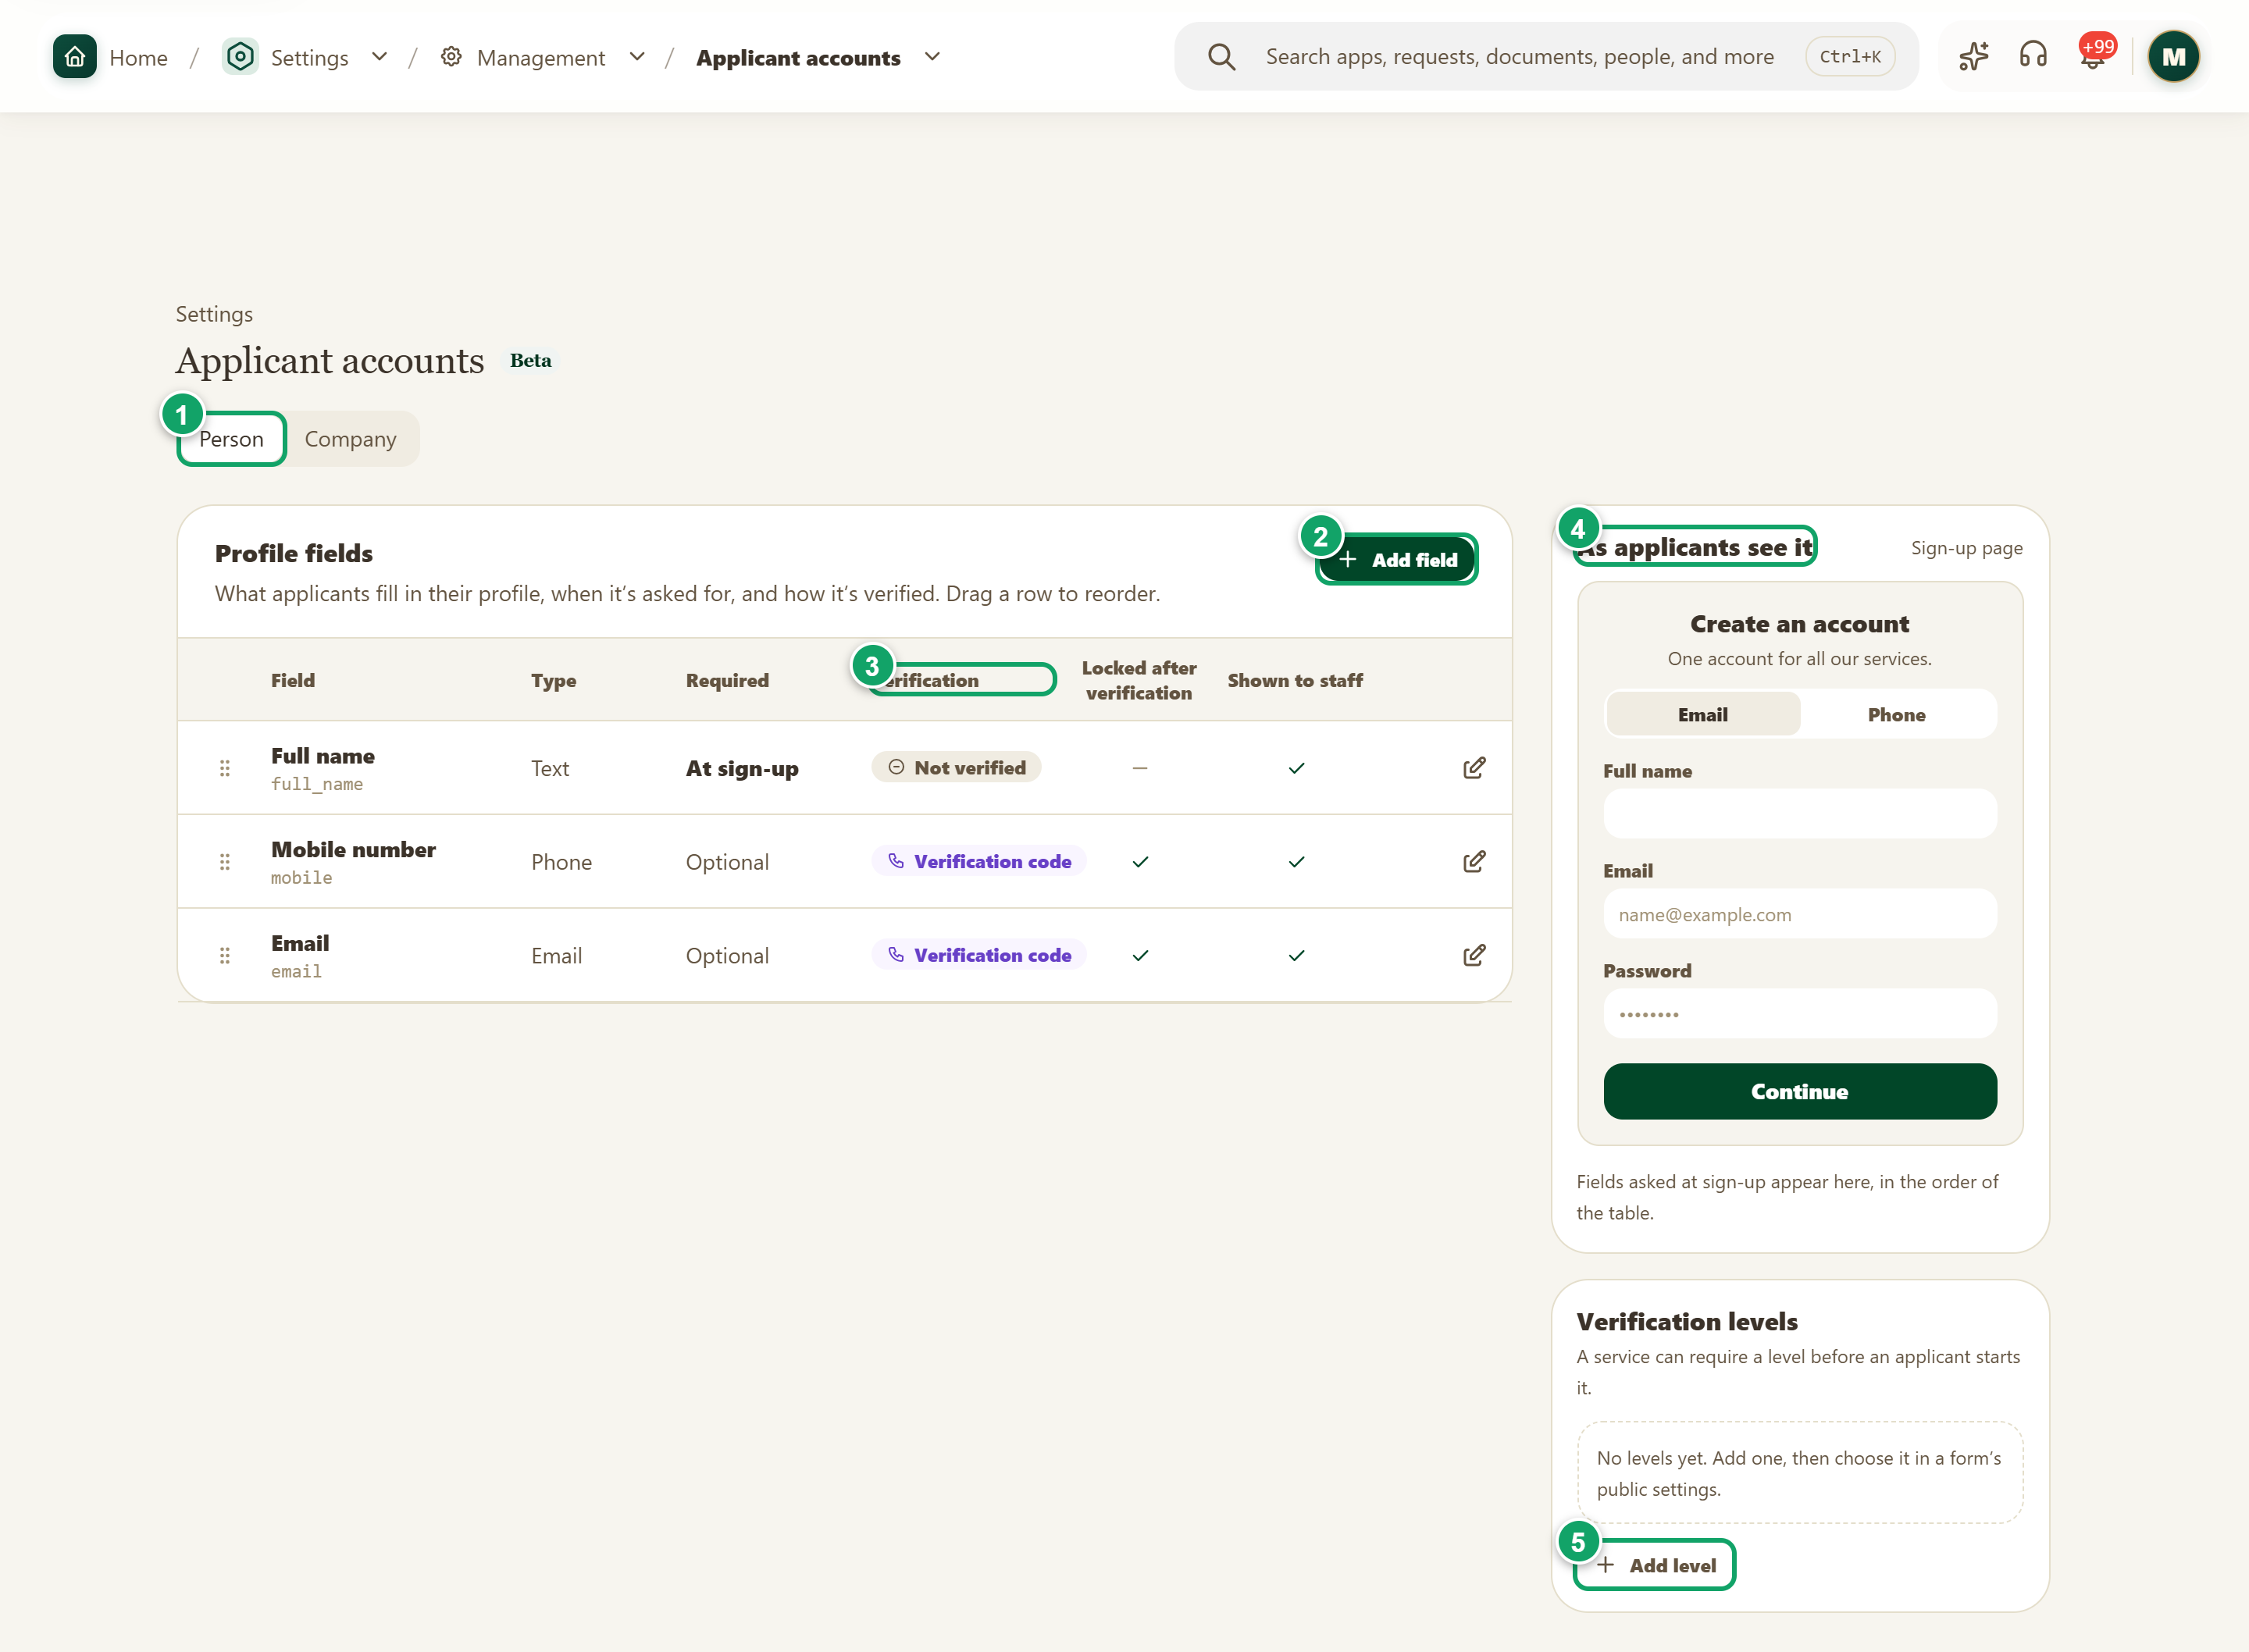
\includegraphics[width=0.95\linewidth,height=0.72\textheight,keepaspectratio]{figures/screens/ch08-applicant-profile-en.png}
\caption{The person profile}
\label{fig:settings-applicant-profile}
\shotnote{The table holds the profile fields, and the card beside it shows their effect on the sign-up page. The test organization has not added verification levels yet. ① “Person”. ② “Add field”. ③ “Verification”: shows how each field’s value is confirmed. ④ “As applicants see it”: a preview of the sign-up page. ⑤ “Add level”.}
\end{figure}

\begin{figure}[H]
\centering
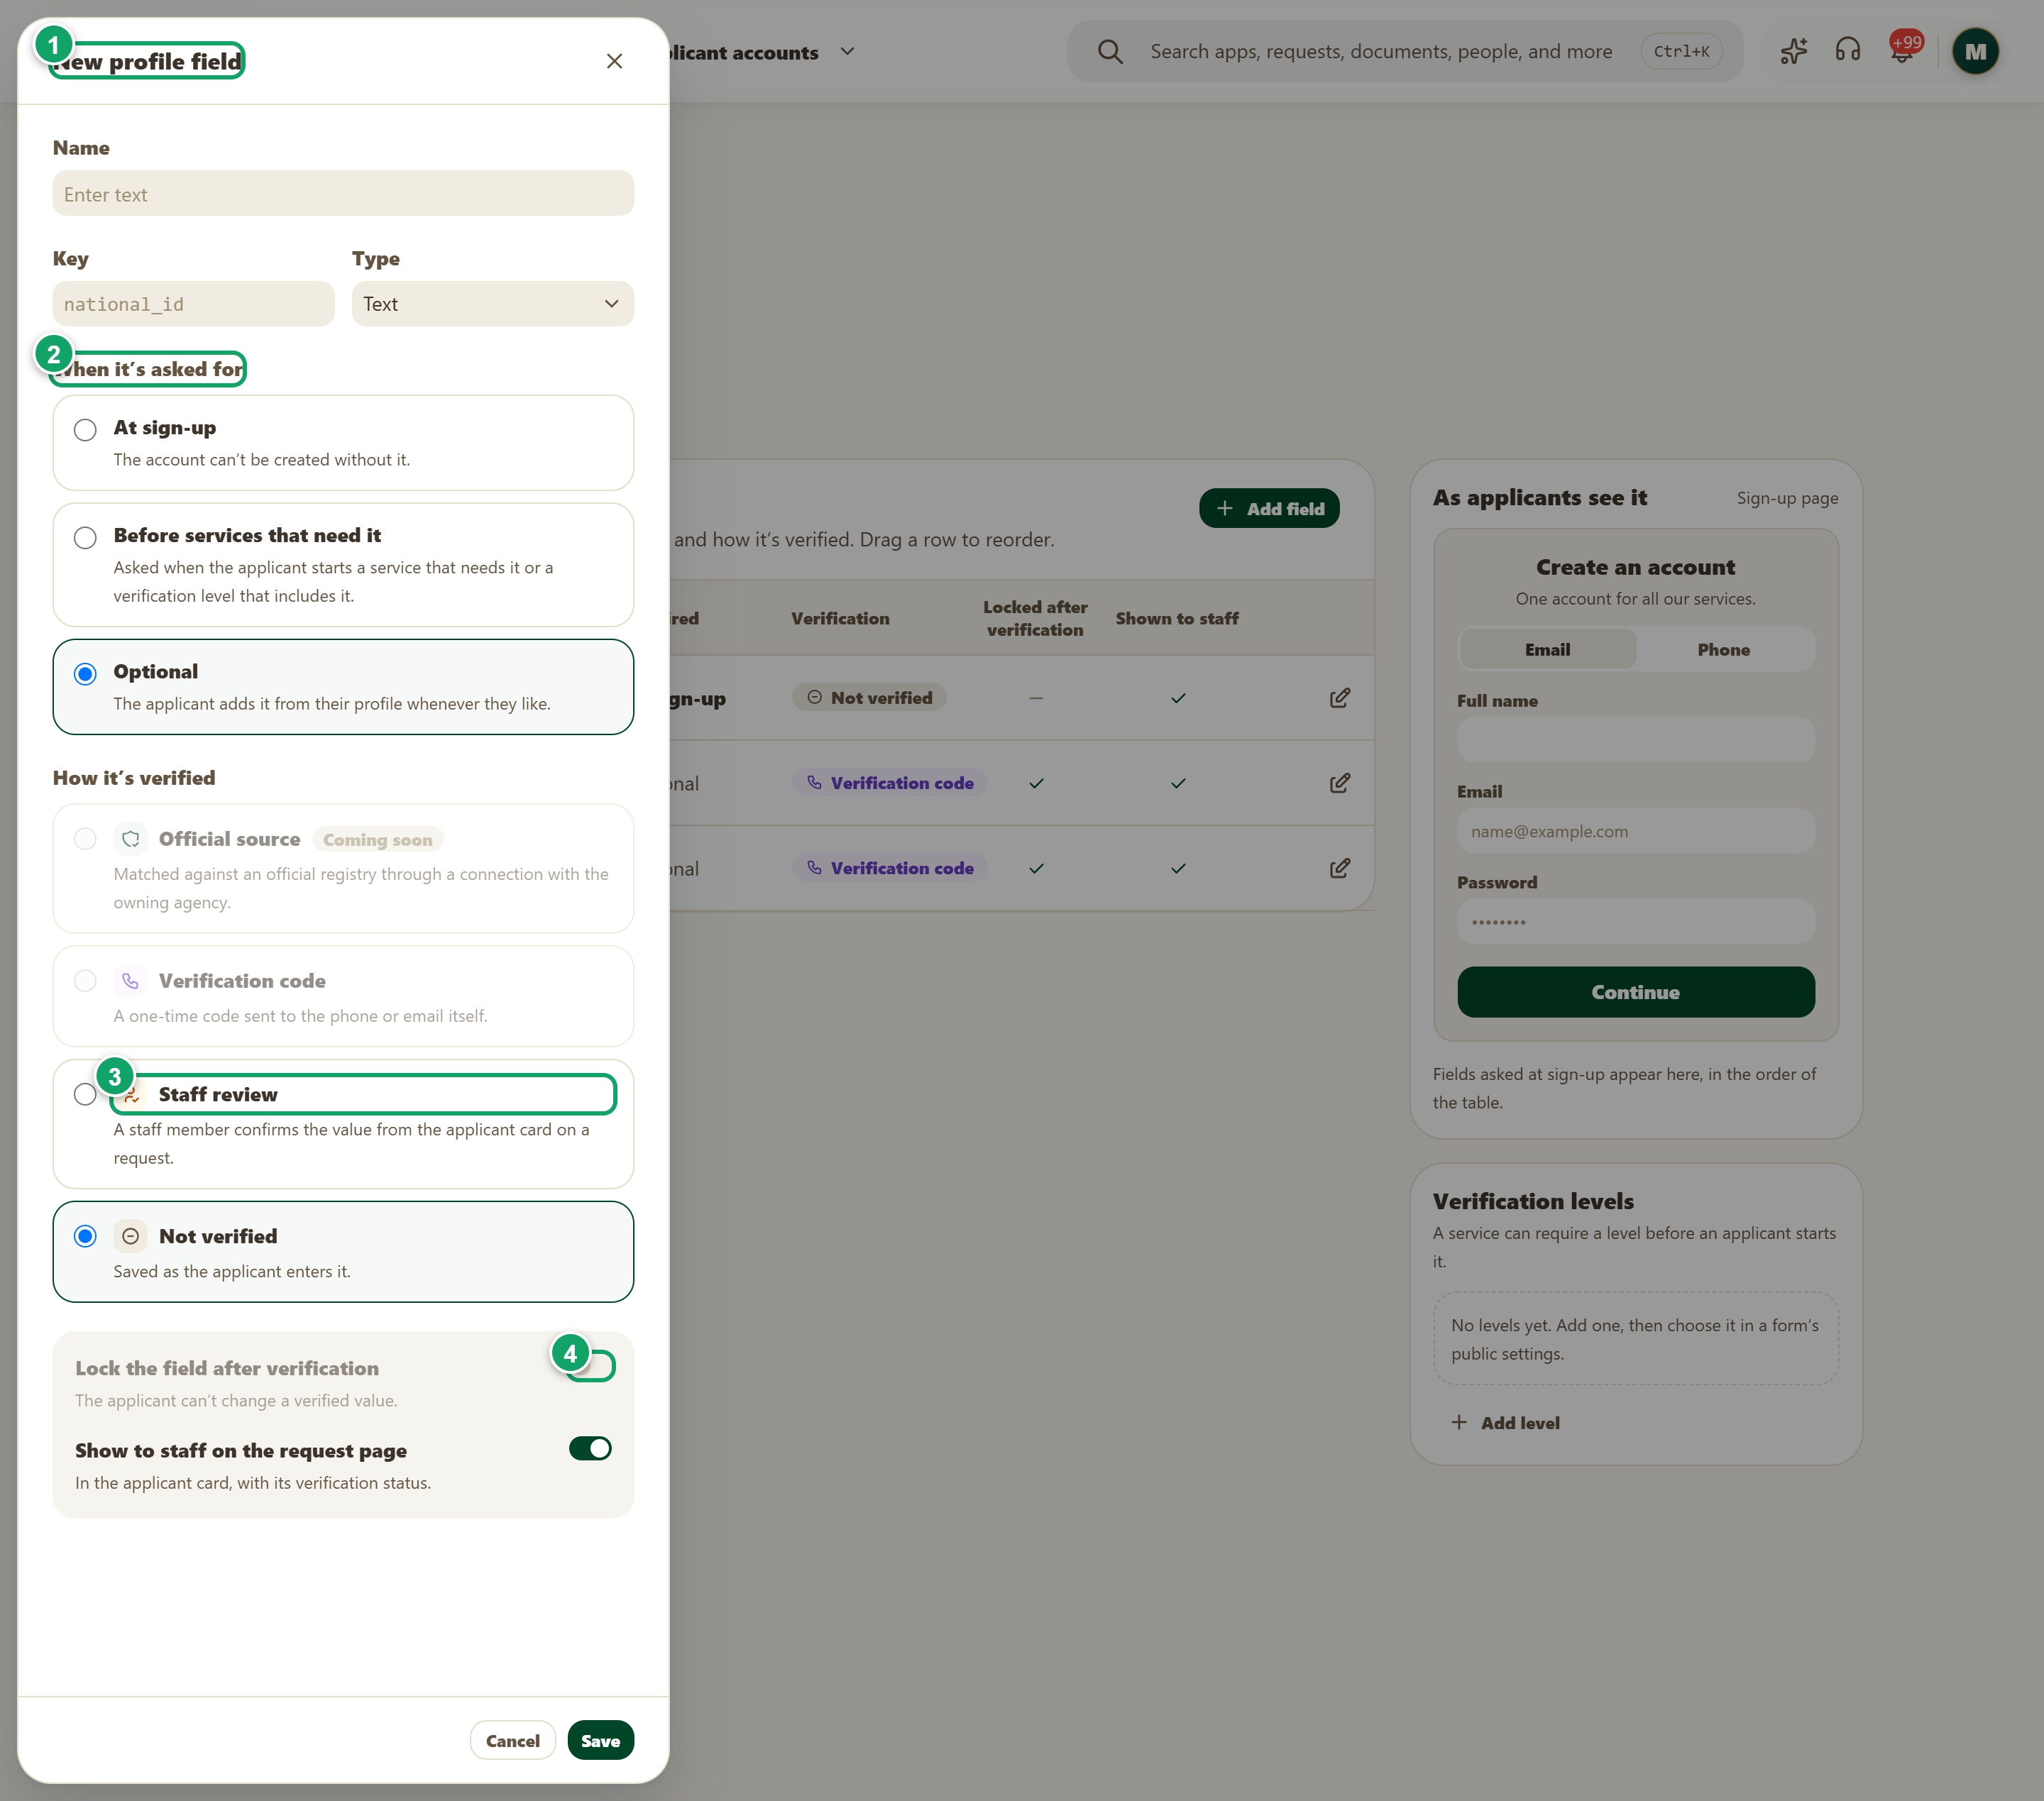
\includegraphics[width=0.95\linewidth,height=0.72\textheight,keepaspectratio]{figures/screens/ch08-applicant-profile-field-en.png}
\caption{The new field form}
\label{fig:settings-applicant-profile-field}
\shotnote{The form opens when you add or edit a field; the image shows it empty and unsaved. Unavailable options are faded: custom fields support only staff review or no verification, and “Official source” is coming later. ① The form’s title. ② “When it’s asked for”. ③ “Staff review”: staff confirm the value from the request page. ④ “Lock the field after verification”: stops the applicant changing a verified value, and does not work with “Not verified”.}
\end{figure}

\begin{figure}[H]
\centering
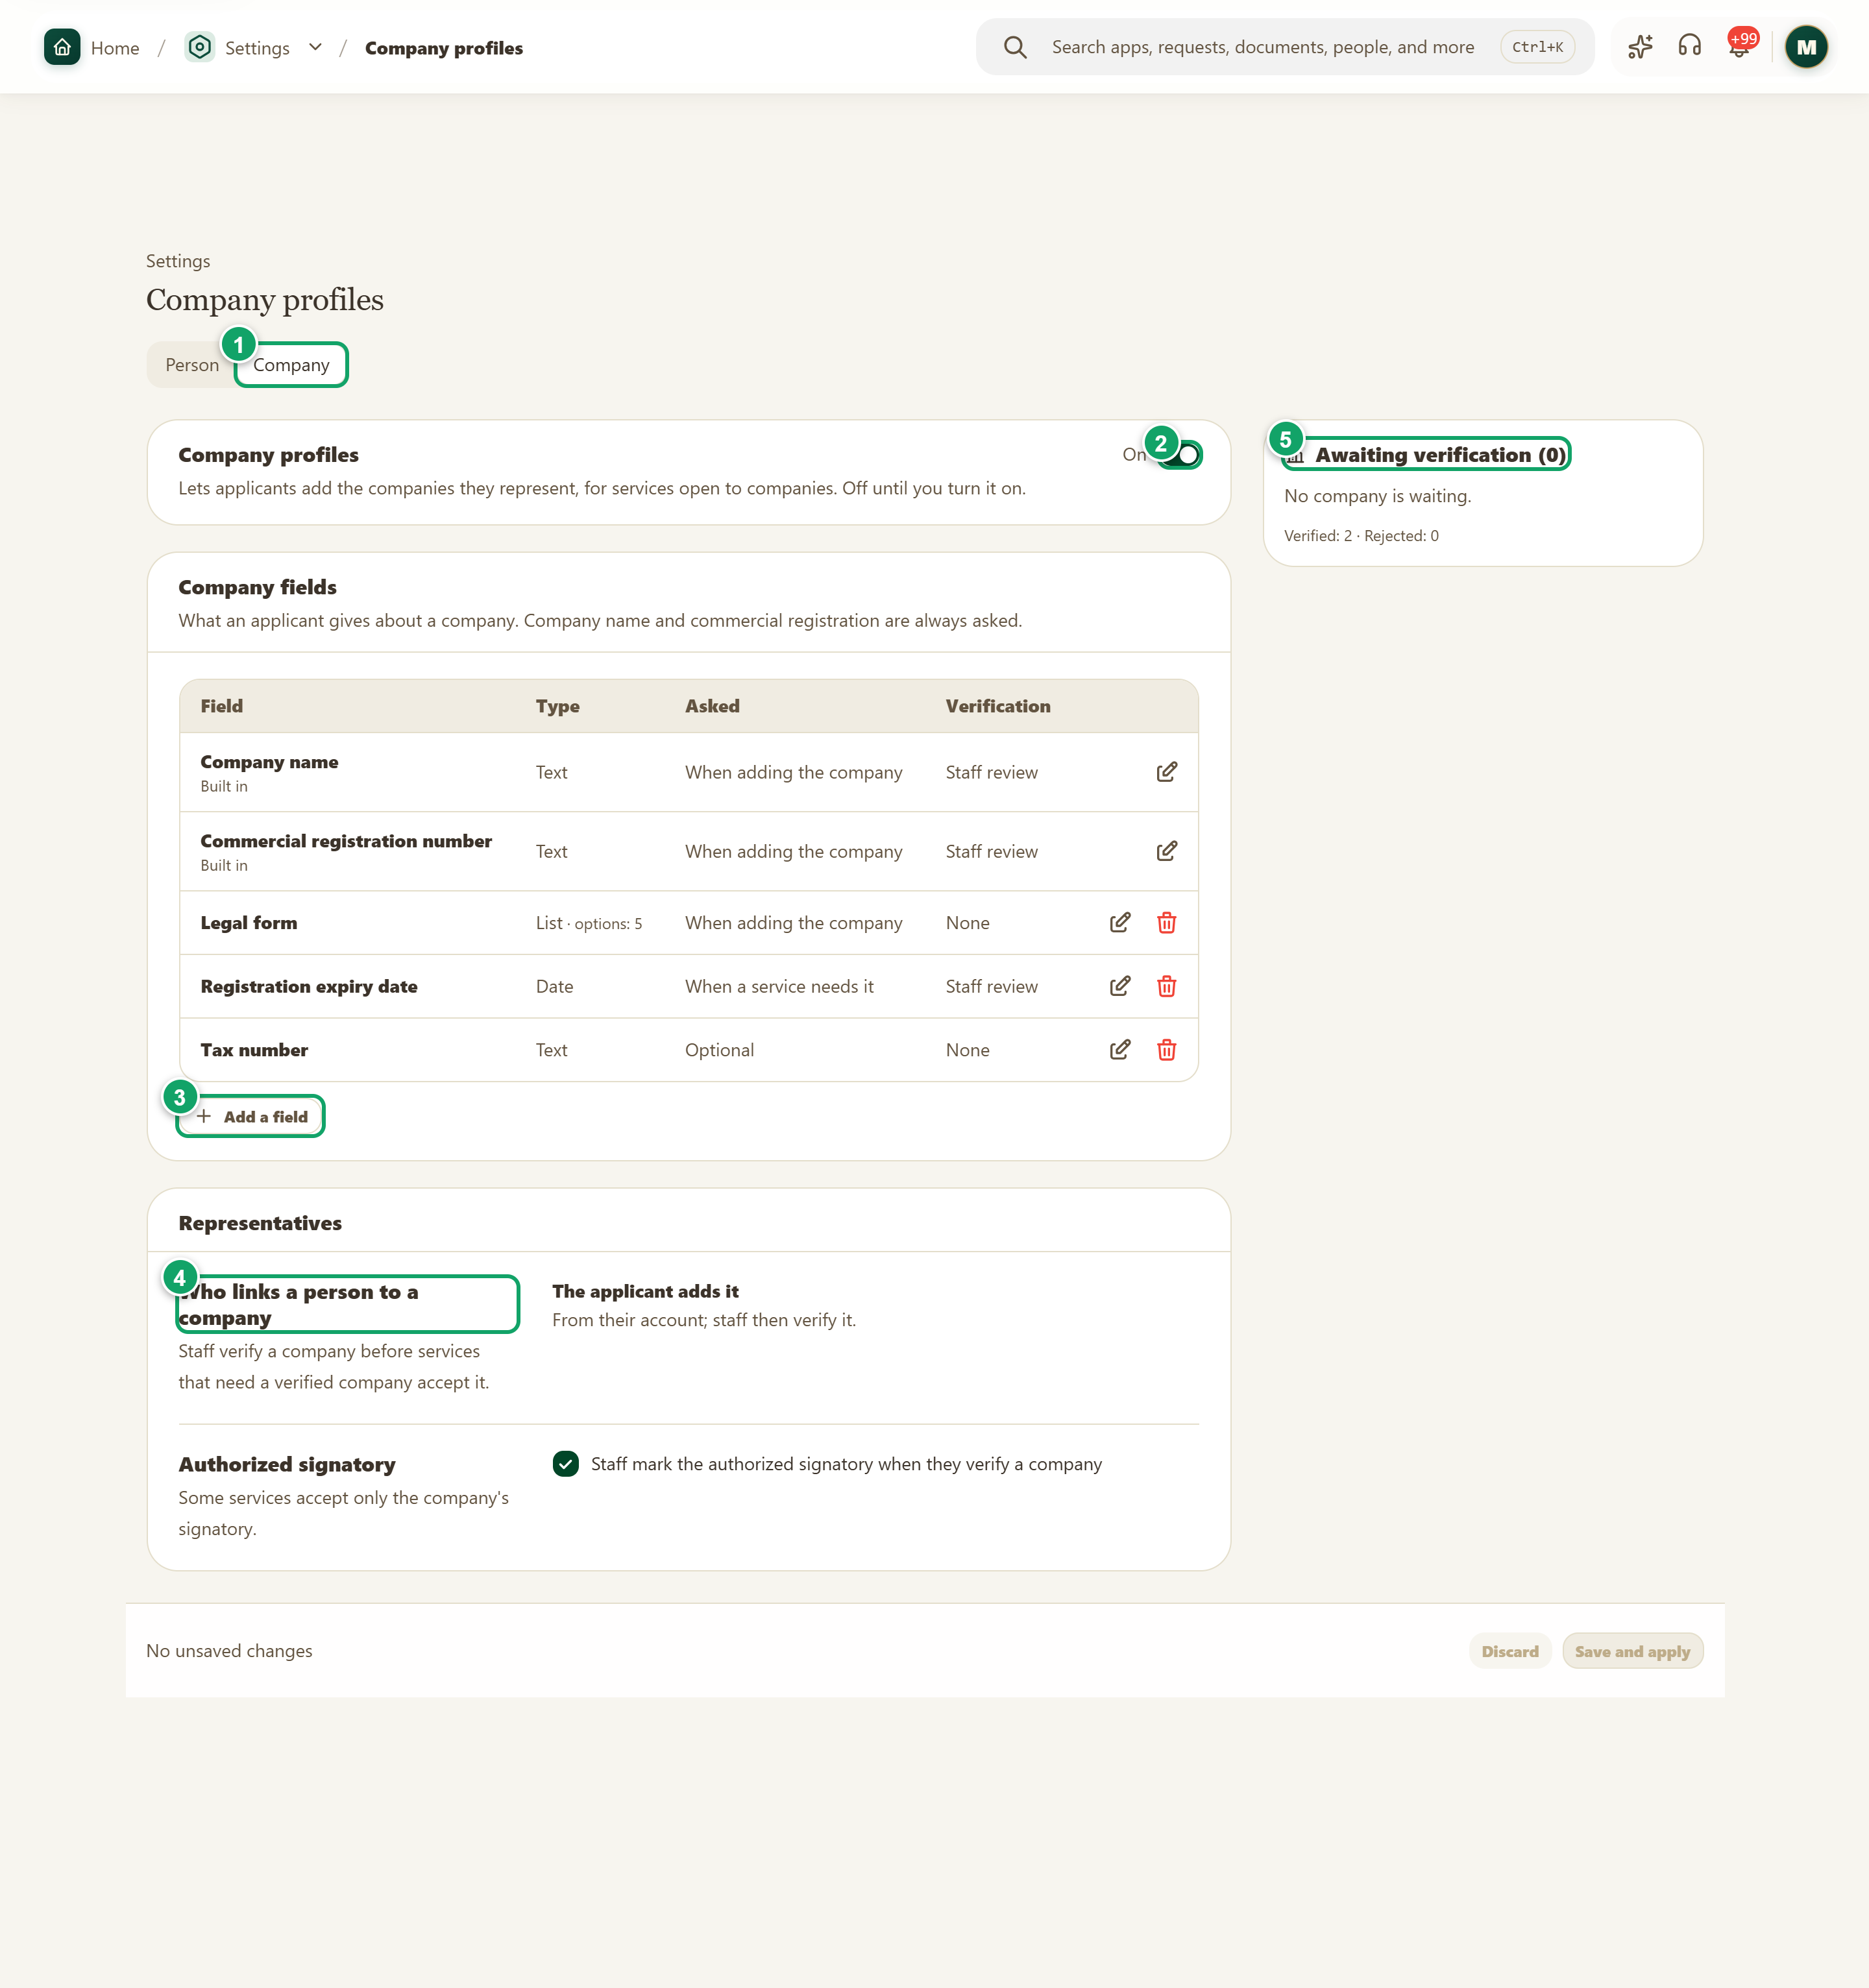
\includegraphics[width=0.95\linewidth,height=0.72\textheight,keepaspectratio]{figures/screens/ch08-applicant-company-en.png}
\caption{The company profile}
\label{fig:settings-applicant-company}
\shotnote{This section is for an applicant who applies on behalf of a company they represent. Staff verify the company first, confirming its details, before services that need a verified company accept it. The data shown belongs to the test organization. ① “Company”. ② The “Company profiles” switch; they stay off until you turn them on. ③ “Add a field”. ④ “Who links a person to a company”. ⑤ “Awaiting verification”: companies waiting for staff review.}
\end{figure}

\begin{table}[H]
\centering
\caption{What do you record in applicant accounts?}
\label{tab:settings-applicant-profile-fields}
\begin{tabularx}{\linewidth}{R{4.2cm} Y}
\rcHeaderRow
\thh{Section} & \thh{What do you record?}\\
“Profile fields” & “Name”, “Key” and “Type”: text, number, date or list. The key is a fixed technical name in English letters that does not change after adding.\\
“When it’s asked for” & “At sign-up”, “Before services that need it” or “Optional”.\\
“Verification” & “Verification code” for phone and email only, “Staff review” and “Not verified”.\\
Extra options & “Lock the field after verification” and “Show to staff on the request page”.\\
“Verification levels” & “Name” and “Fields the level needs”. Each must be filled in, and verified if it has a verification method.\\
“Company” & Turning it on, “Company fields” up to 20, the option to name the “Authorized signatory” at verification, and reviewing waiting companies by verifying or rejecting them.\\
\end{tabularx}
\end{table}

\begin{enumerate}
\item Open “Settings”, then “Applicant accounts”.
\item Press “Add field”, write the name and key, and choose the type.
\item Set “When it’s asked for” and “Verification”, then press “Save”.
\item Drag a field’s row to change its order; the order saves at once.
\item Press “Add level”, name it, choose its fields and press “Save”. Then choose the level in the service’s public form settings.
\item If you deal with companies, open “Company”, turn on “Company profiles”, then press “Save and apply”.
\end{enumerate}

\textbf{Check:} The field appears in the table, and if you chose “At sign-up” it also appears under “As applicants see it”. Note that a level’s delete button acts at once without asking. Deleting a field keeps the saved values, but they no longer show or get asked for.

\clearpage
\section{Messages}
\label{sec:settings-feature-messages}

This page decides what applicants and outside parties are told, over which channels, and keeps a log of everything sent. A channel is how the message reaches them: SMS, WhatsApp, email or a portal notification. A variable is a slot in the text, such as the request number, that the system replaces with the real value when sending.

Use this page when launching a new service, when changing a message’s text or a sending rule, or to find out why a message did not arrive. The organization owner and holders of the Administrator role open it. A role may also let another member manage follow-up templates or view the log only, and that member sees just those parts.

\begin{rcnote}[Example: Horizon]
Horizon’s system administrator reviews the “Action needed from you” event at ②, opens the email channel at ③, edits the text and saves it at ⑤. When Sarah Al-Khatib asks why an email did not reach an applicant, he opens “Log” and reads the message’s status.
\end{rcnote}
\begin{figure}[H]
\centering
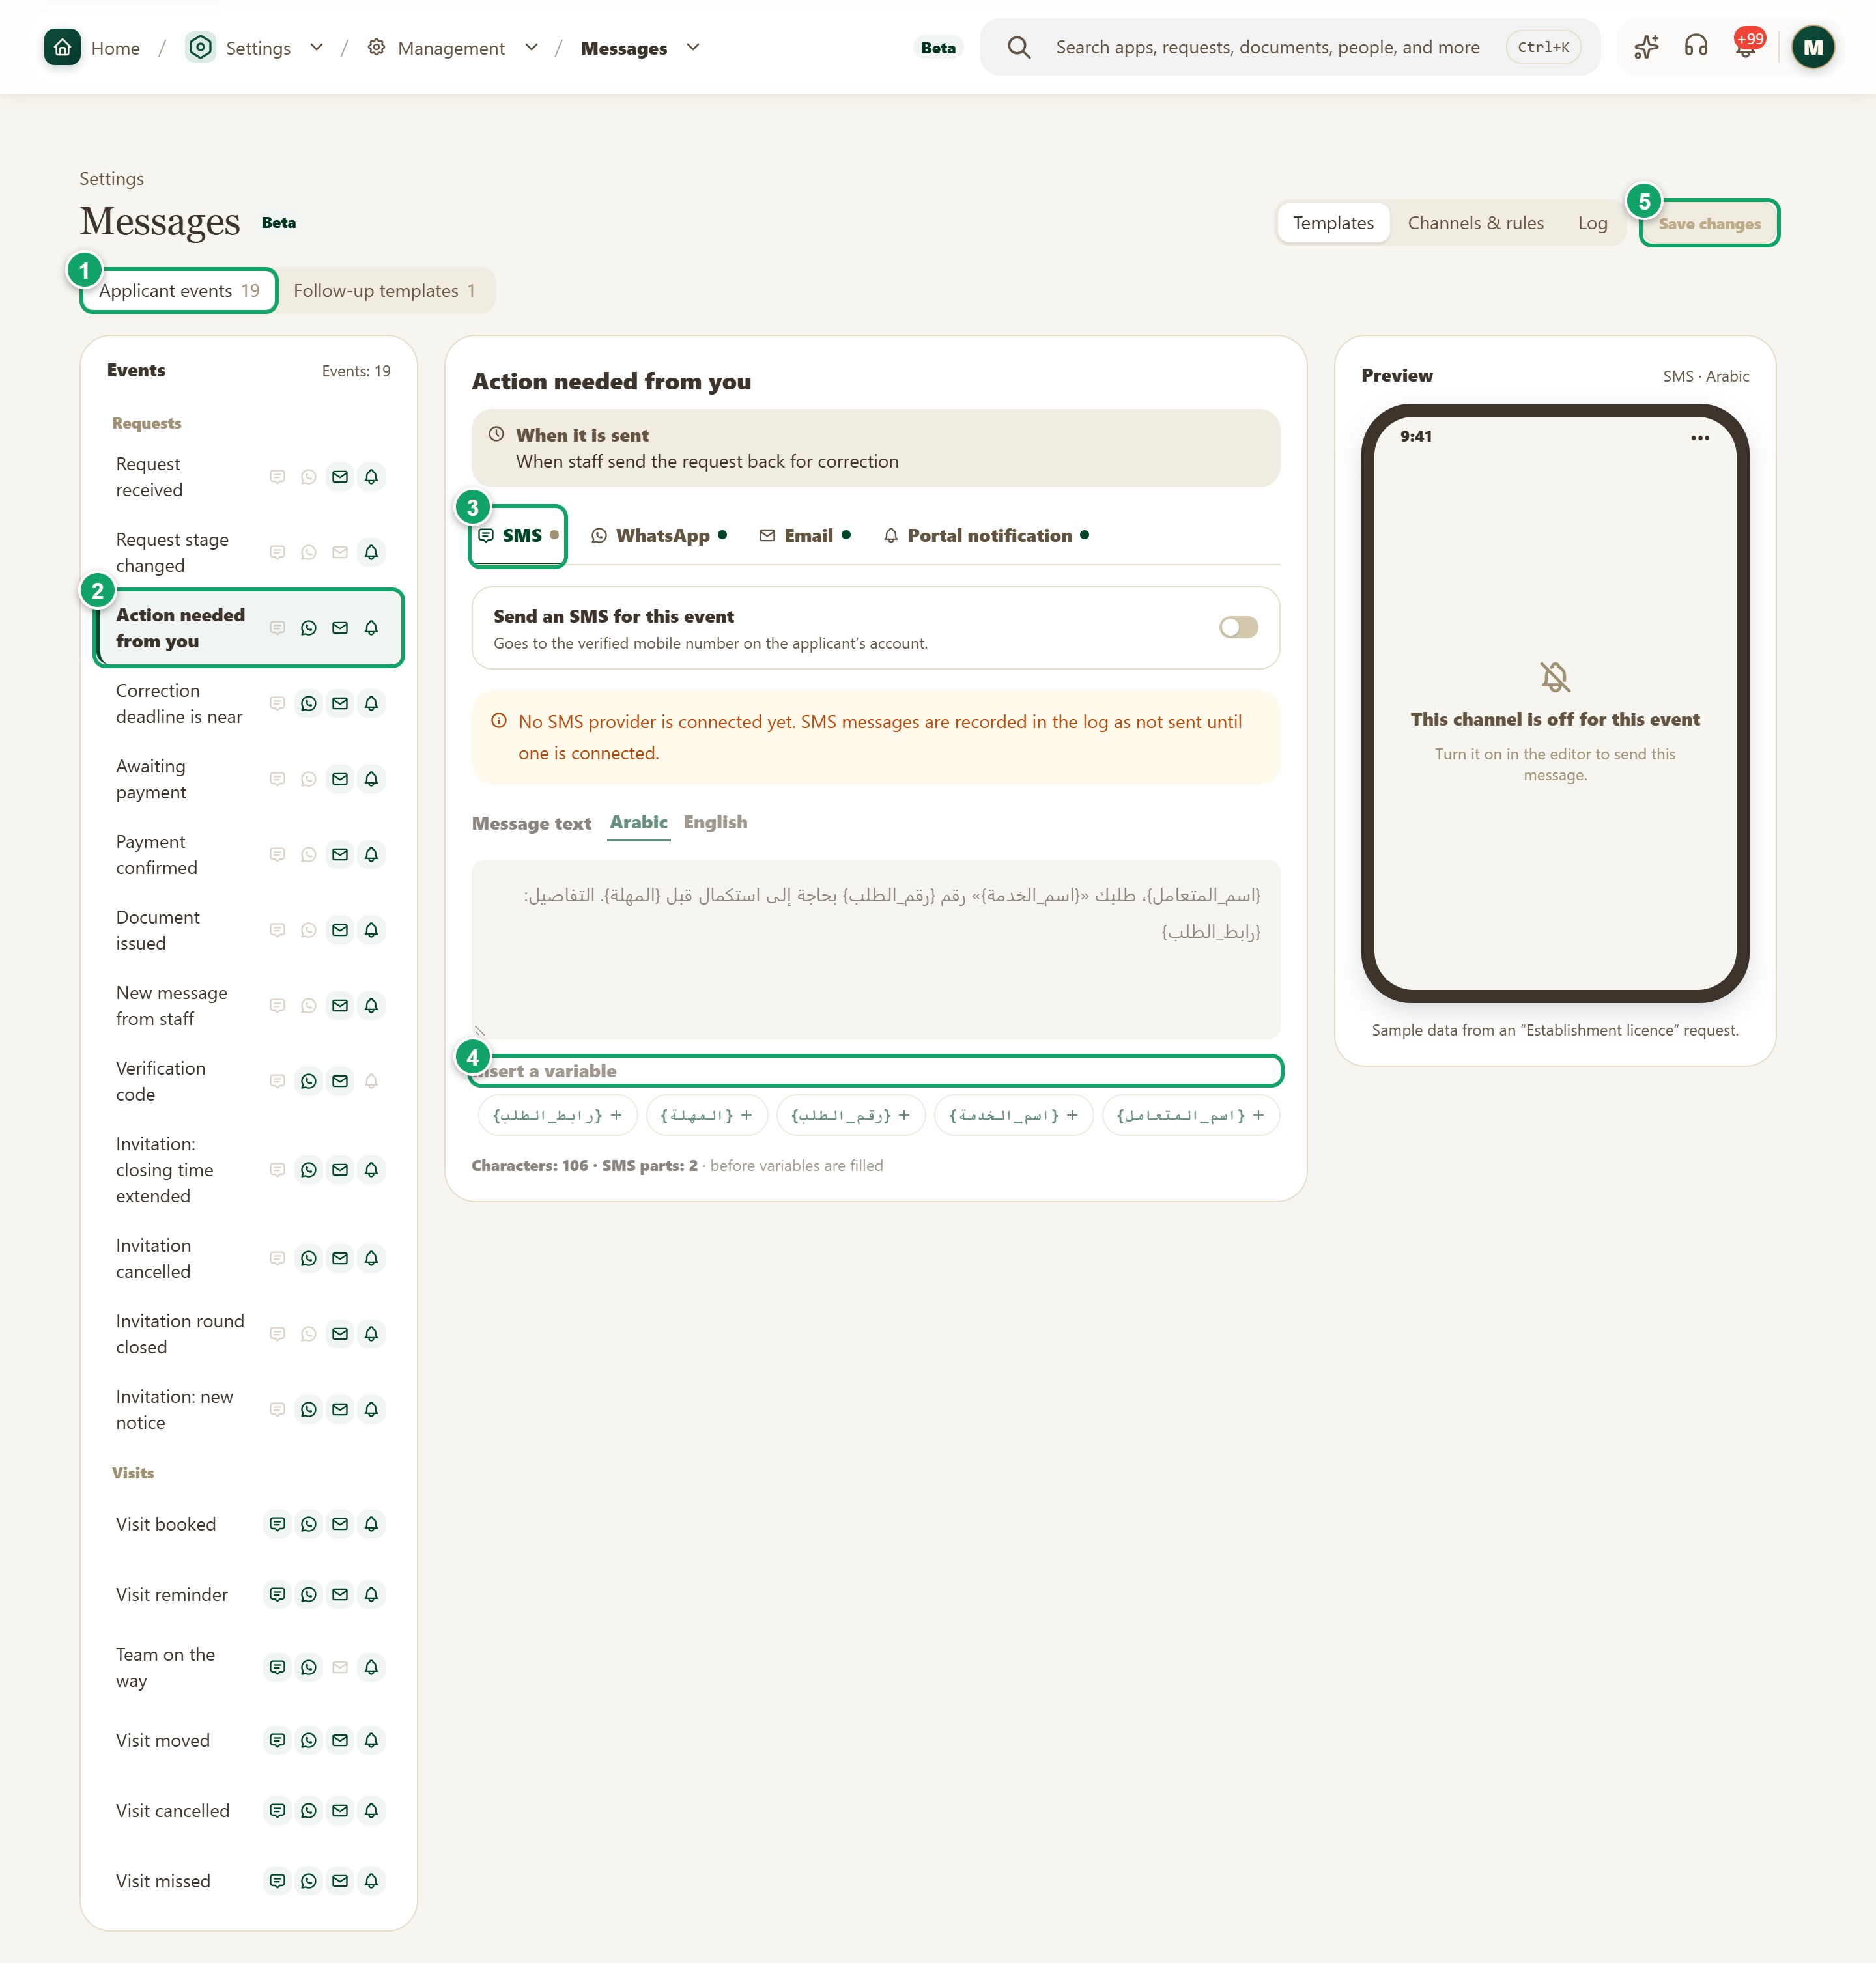
\includegraphics[width=0.95\linewidth,height=0.72\textheight,keepaspectratio]{figures/screens/ch08-messages-templates-en.png}
\caption{Applicant events}
\label{fig:settings-messages-templates}
\shotnote{An event is what makes the system send a message, such as receiving a request or moving a visit. The list shows all nineteen events, each row shows its enabled channels, and the preview shows how the message looks. ① “Applicant events”. ② The selected event. ③ The selected channel. ④ “Insert a variable”: places a changing value in the text. ⑤ “Save changes”.}
\end{figure}

\begin{figure}[H]
\centering
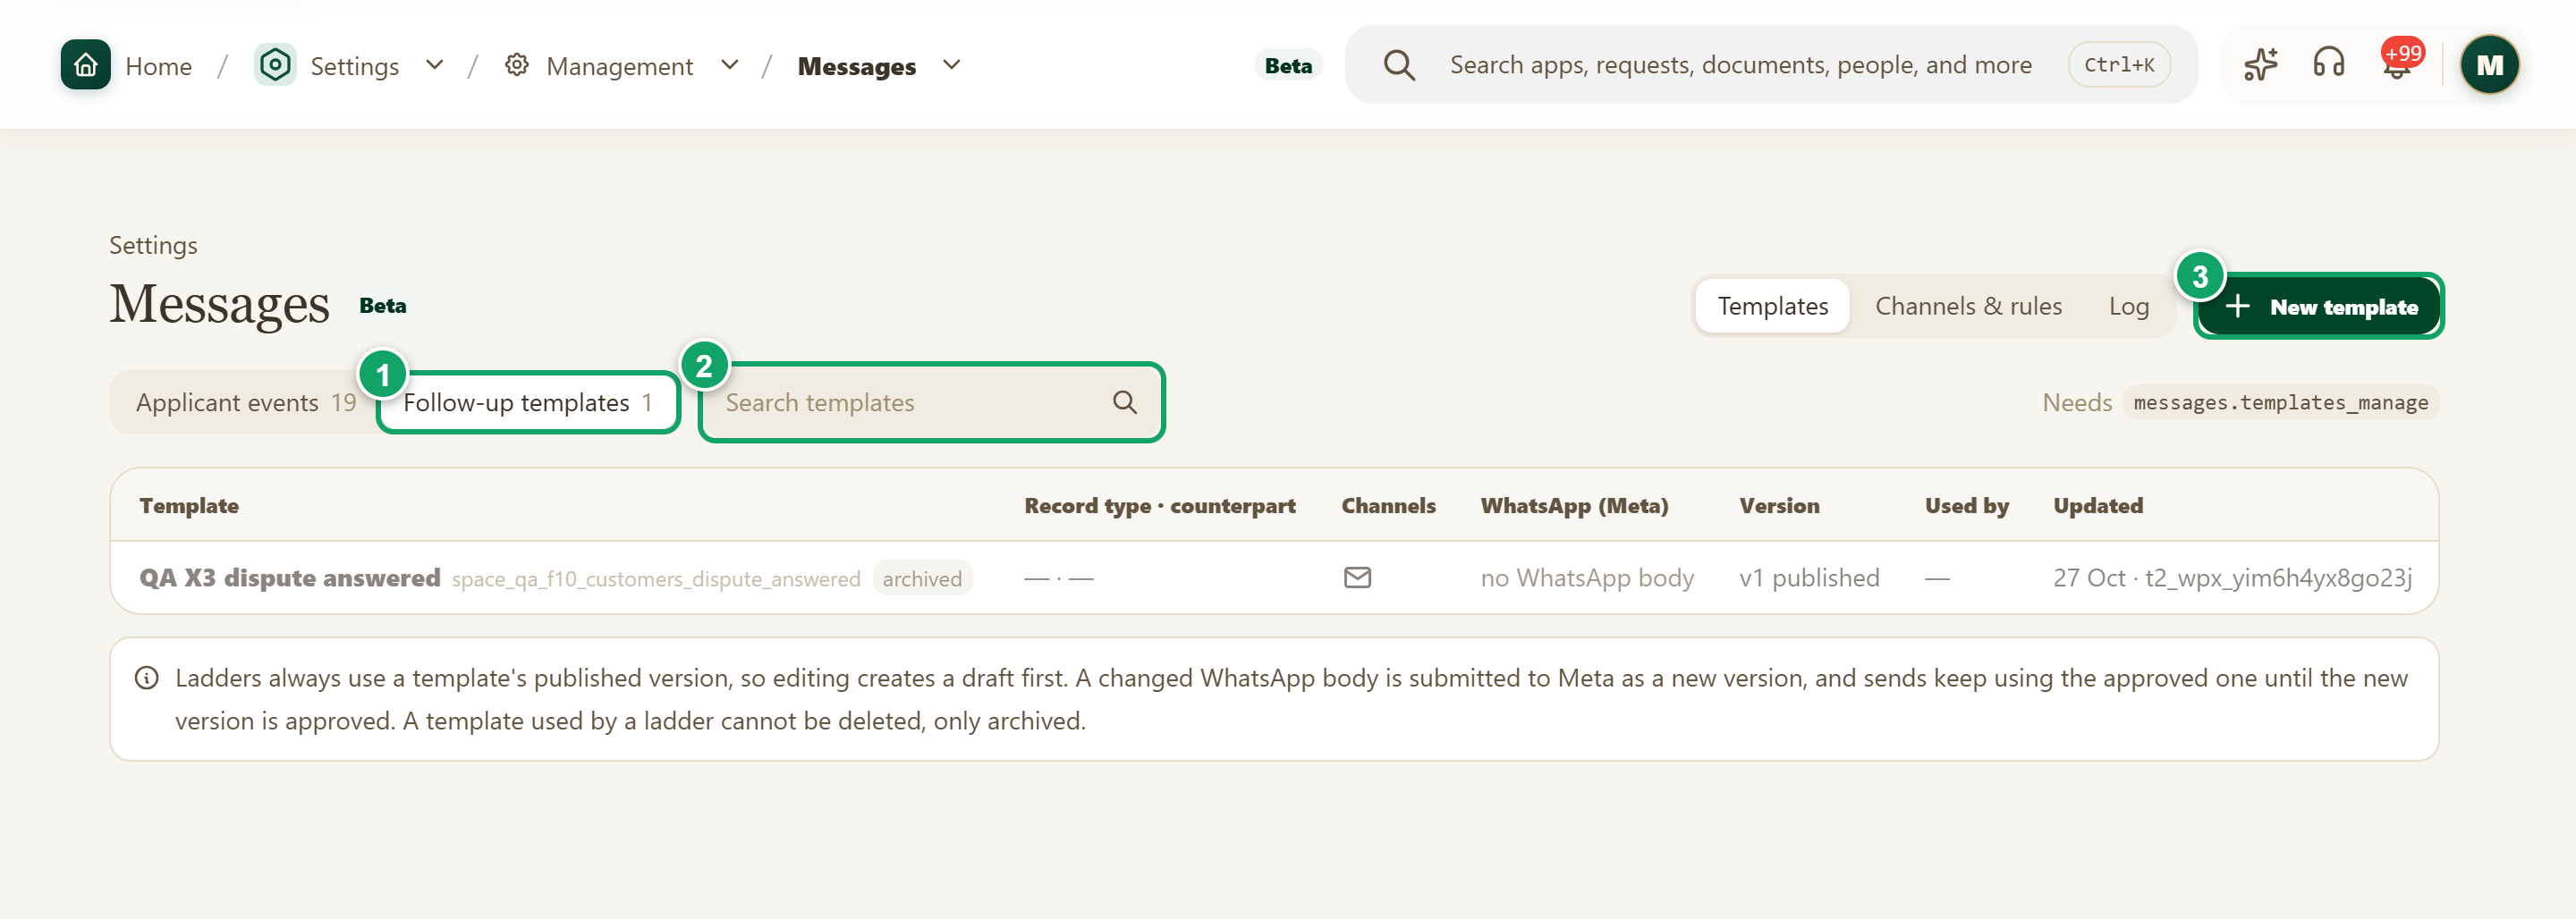
\includegraphics[width=0.95\linewidth,height=0.72\textheight,keepaspectratio]{figures/screens/ch08-messages-followup-en.png}
\caption{Follow-up templates}
\label{fig:settings-messages-followup}
\shotnote{A follow-up template is a message sent by a step in a ladder, a sequence of reminders that follows up a party until the task is done, such as reminding a customer of an invoice due. The published version is always the one sent, so every edit starts as a draft. ① “Follow-up templates”. ② The search field. ③ “New template”.}
\end{figure}

\begin{figure}[H]
\centering
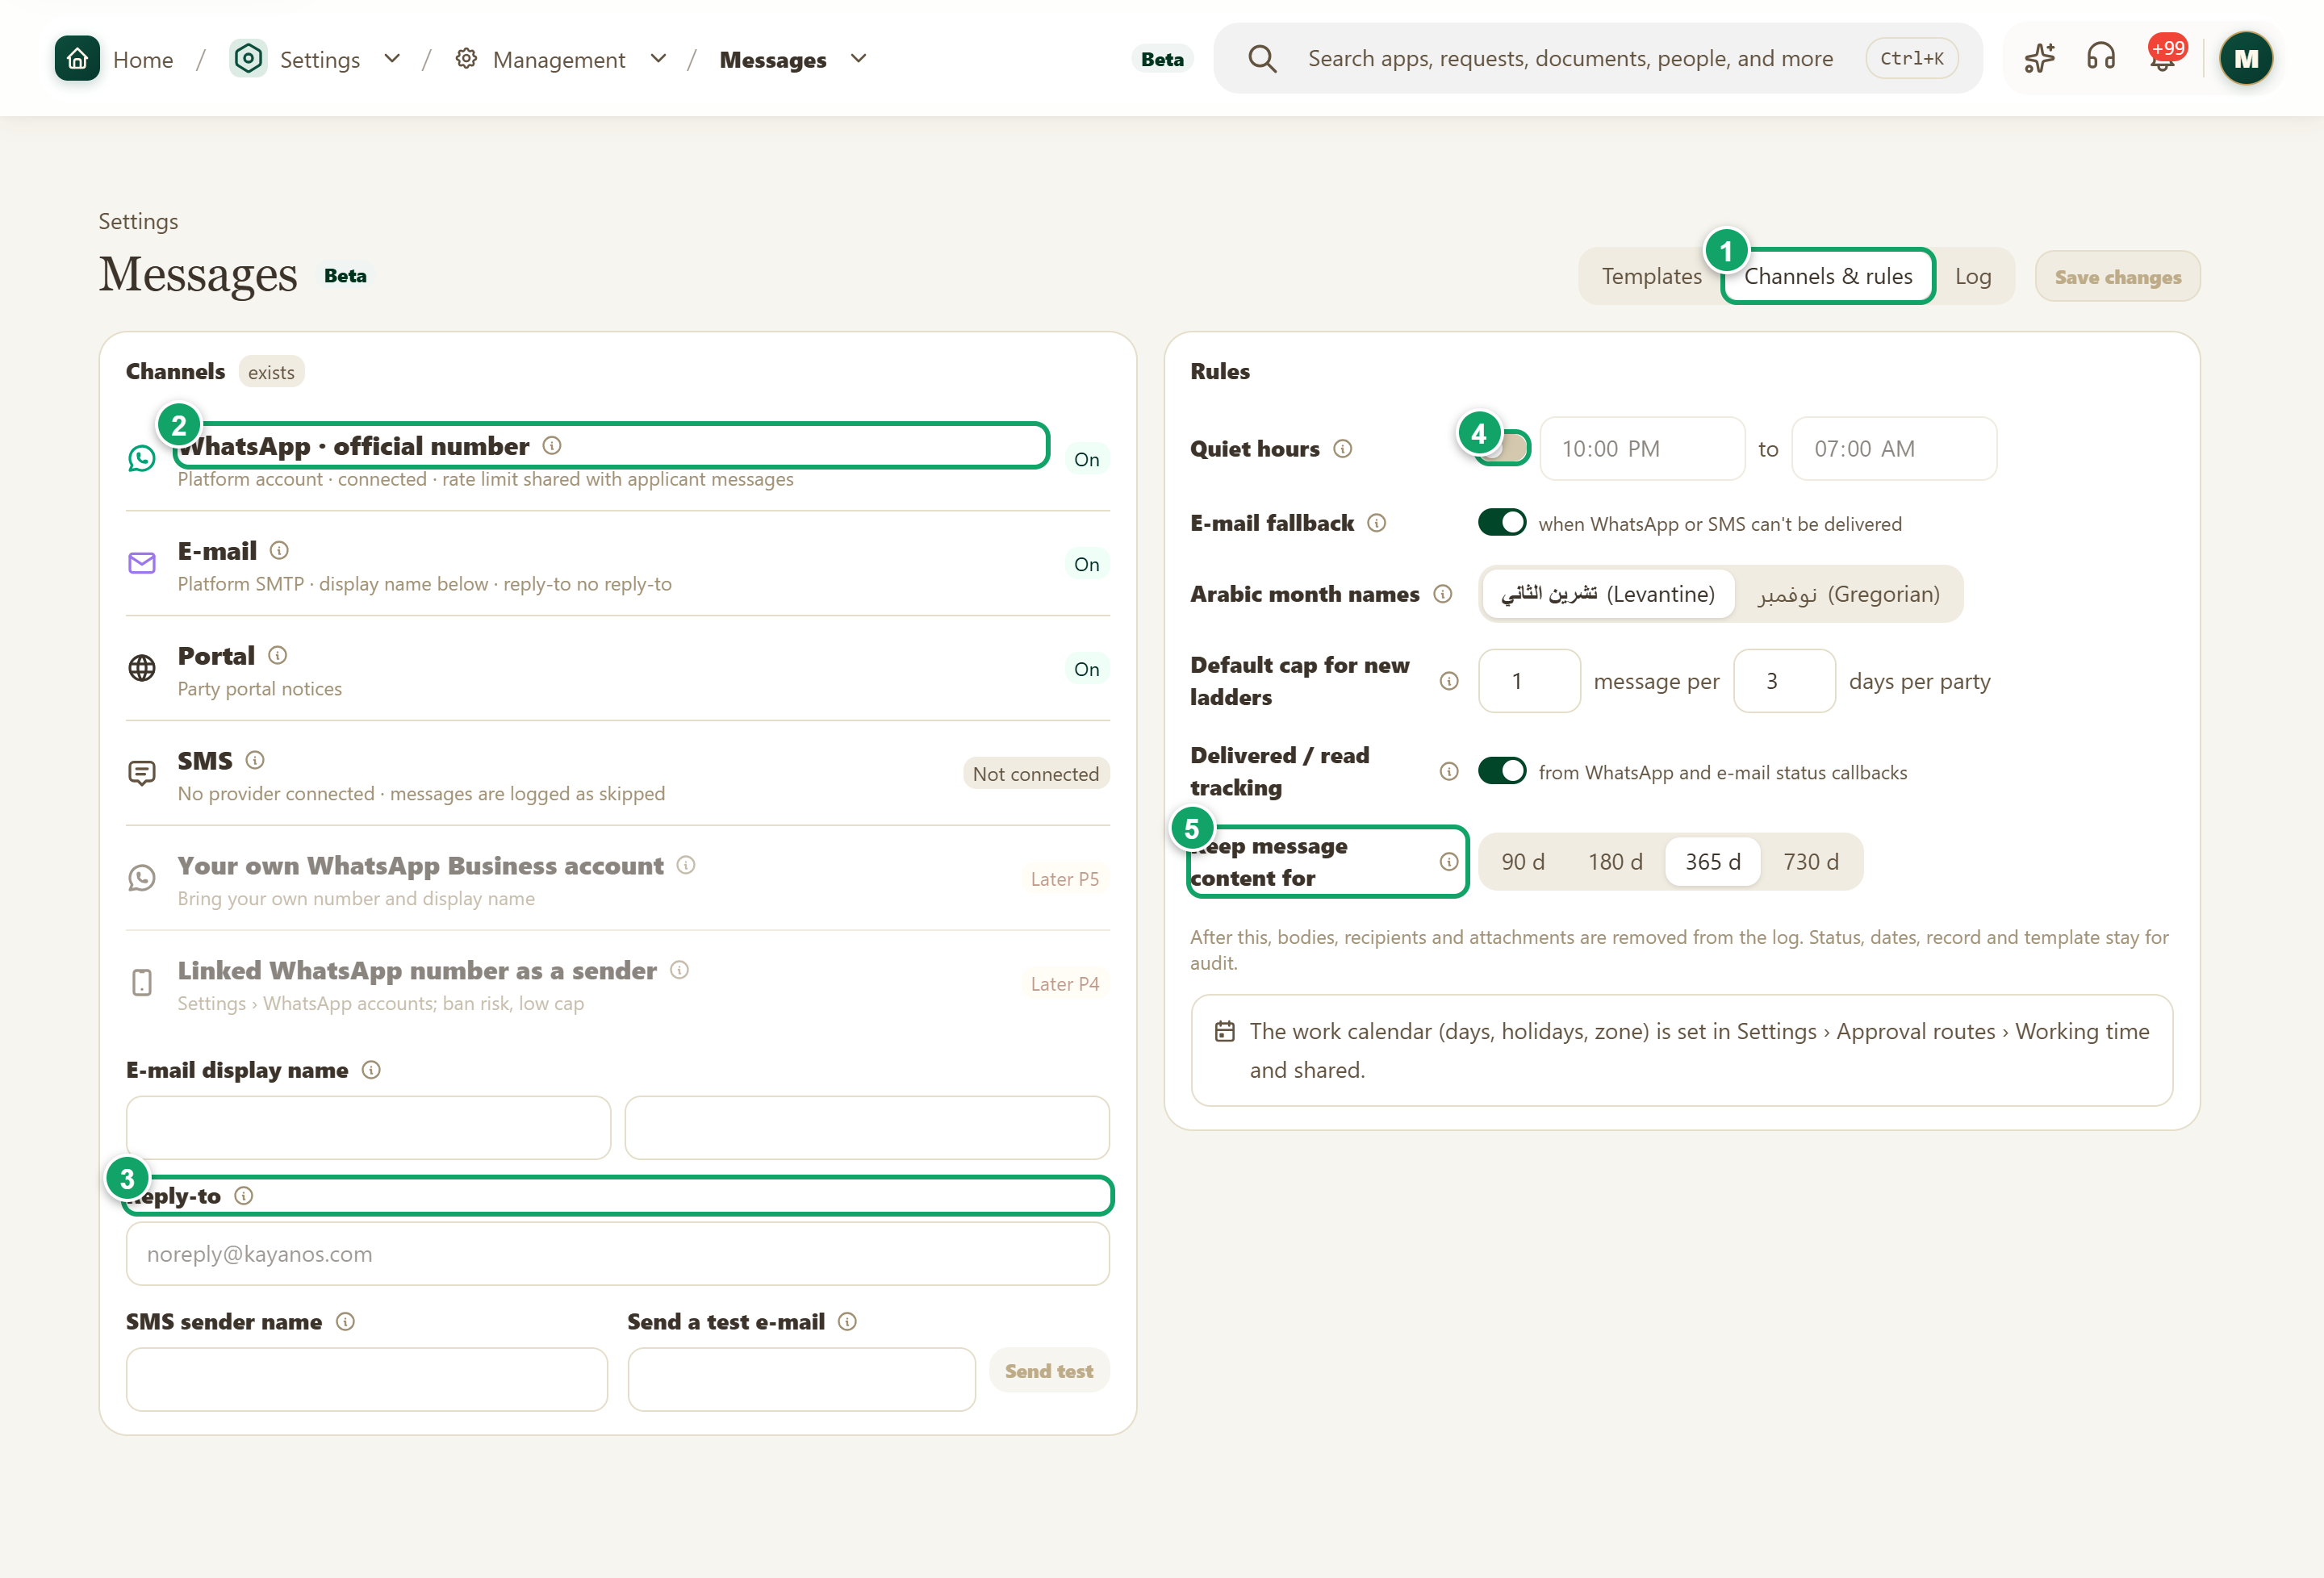
\includegraphics[width=0.95\linewidth,height=0.72\textheight,keepaspectratio]{figures/screens/ch08-messages-channels-en.png}
\caption{Channels and rules}
\label{fig:settings-messages-channels}
\shotnote{This page brings together the channels’ status and the rules that apply to messages. The test organization has no SMS provider, so those messages are logged as “Skipped” and reach nobody. ① “Channels \& rules”. ② “WhatsApp · official number”: the number these messages are sent from. ③ “Reply-to”: use a mailbox someone reads; if you leave it empty, replies go nowhere. ④ The “Quiet hours” switch: messages due during these hours wait until they end. ⑤ “Keep message content for”.}
\end{figure}

\begin{figure}[H]
\centering
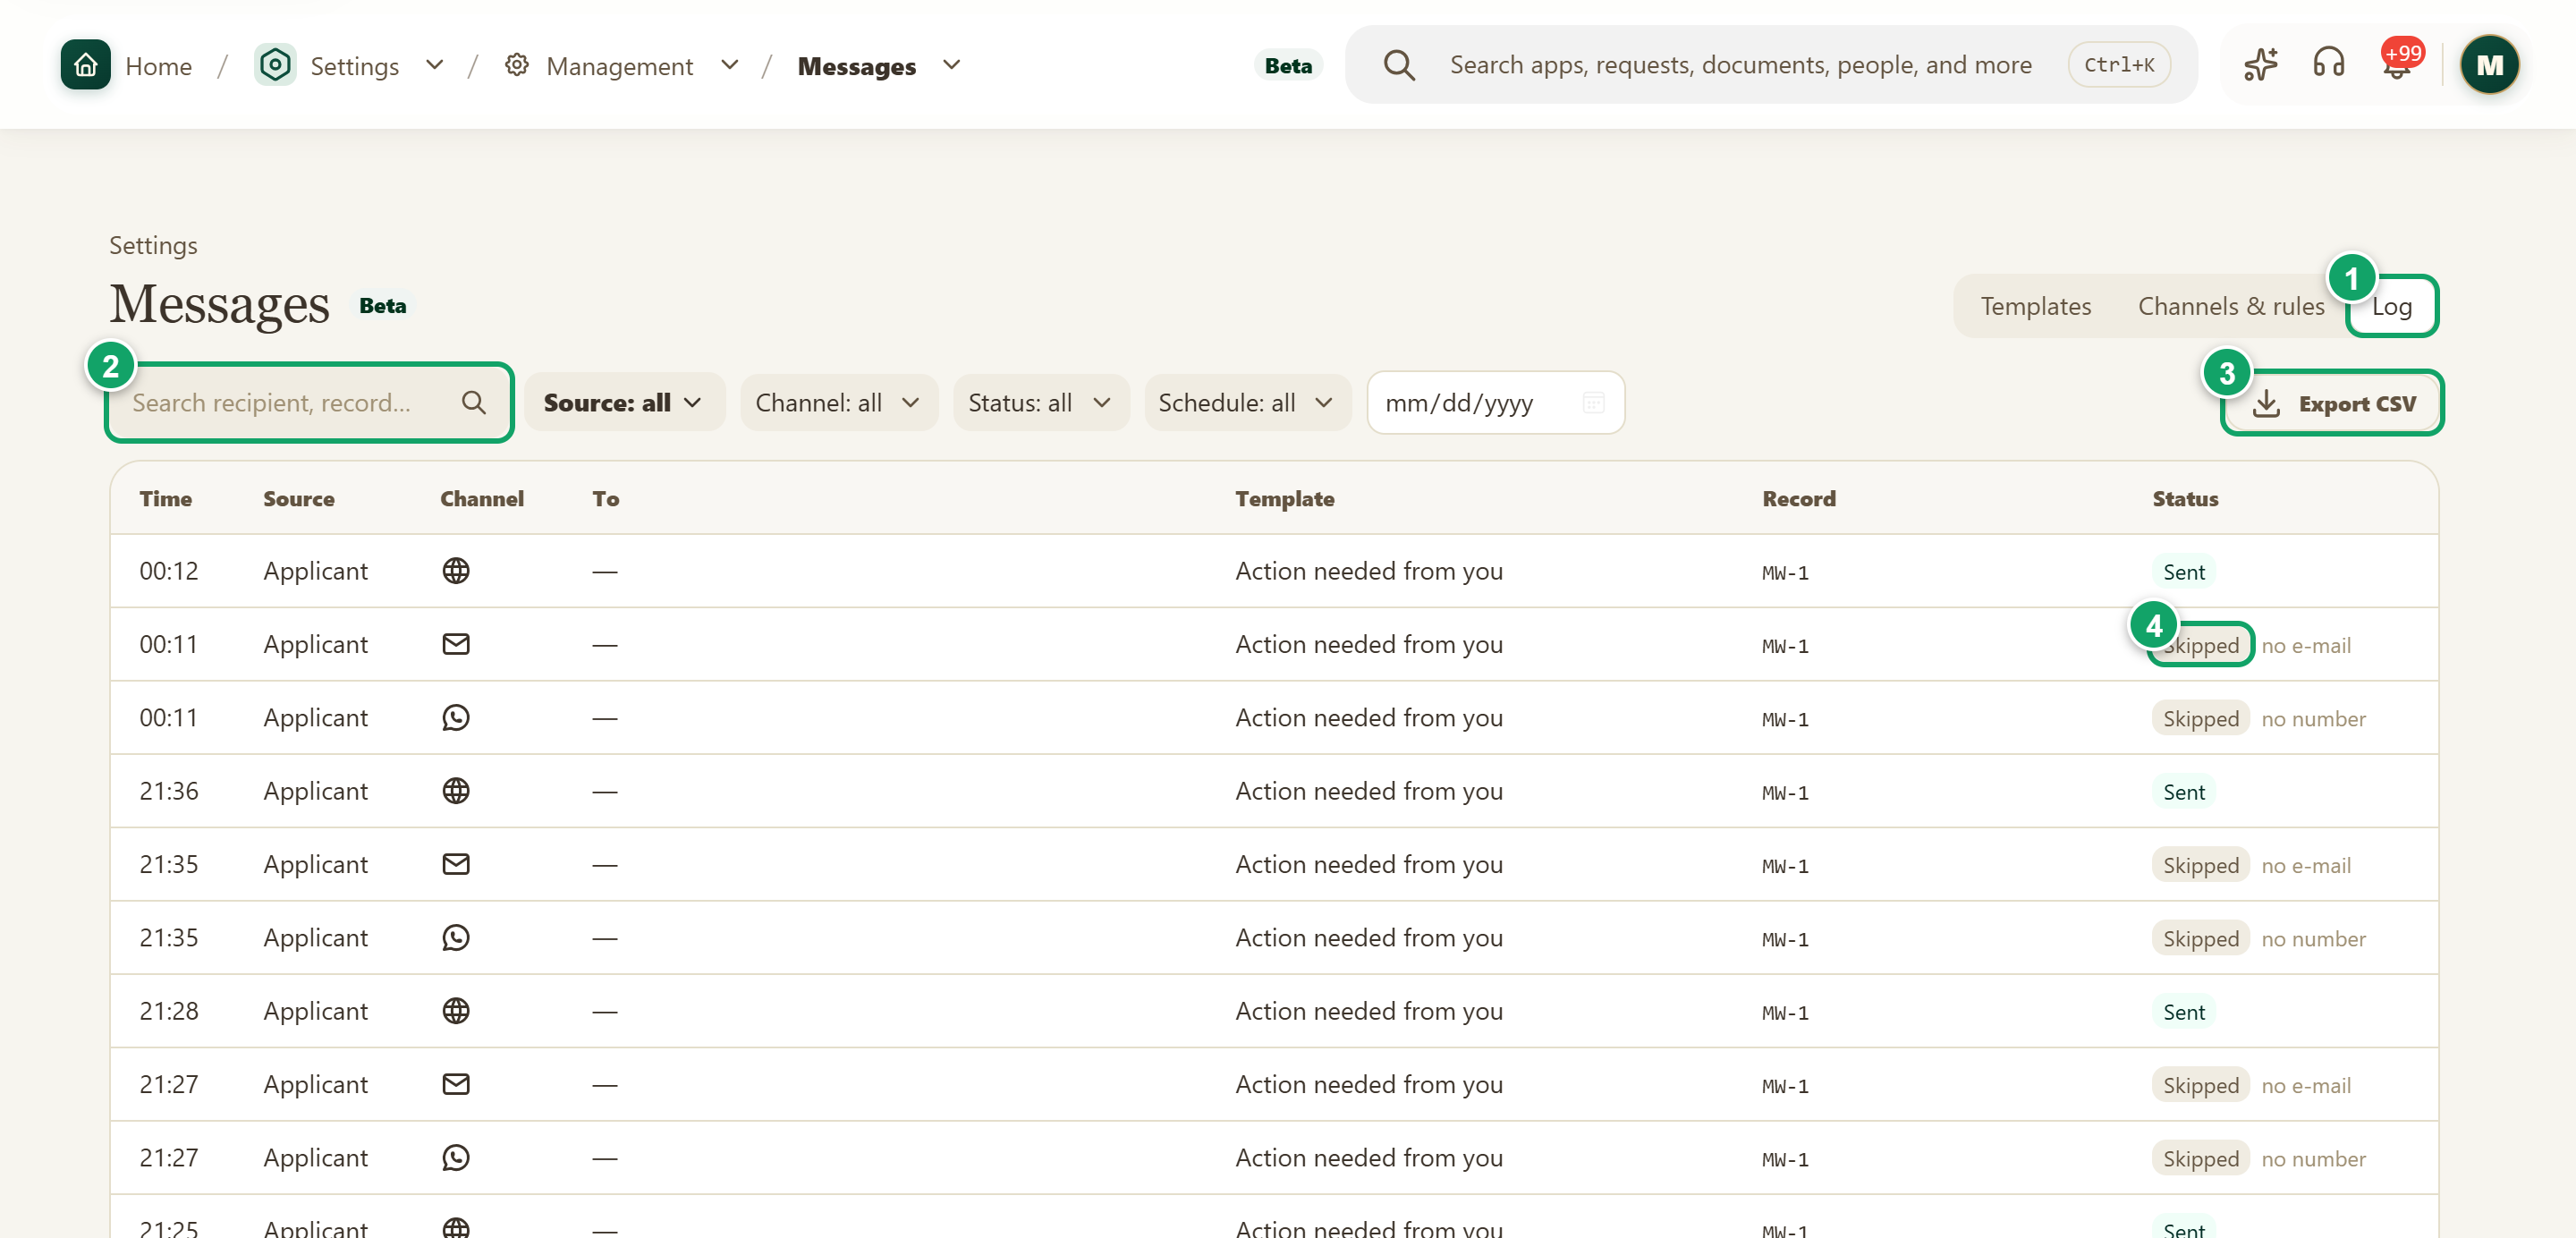
\includegraphics[width=0.95\linewidth,height=0.72\textheight,keepaspectratio]{figures/screens/ch08-messages-log-en.png}
\caption{The message log}
\label{fig:settings-messages-log}
\shotnote{The log records each sending attempt, its channel and its status, so you can tell whether a message was sent and why not. The rows shown are test data. ① “Log”. ② The field to search for a recipient or record. ③ “Export CSV”: saves the results to a file. ④ “Skipped”: the message was not sent, and the reason appears beside the status.}
\end{figure}

\begin{table}[H]
\centering
\caption{What do you record in messages?}
\label{tab:settings-messages-fields}
\begin{tabularx}{\linewidth}{R{4.2cm} Y}
\rcHeaderRow
\thh{Section} & \thh{What do you record?}\\
“Applicant events” & For each event and channel: turning sending on or off, the Arabic and English text, and “Restore the default text” after editing. For the visit reminder you set the days before and the time.\\
Not edited here & WhatsApp text in events is an approved template edited outside this page. The “Verification code” event is shown for reference only.\\
“Follow-up templates” & The key, name, record type and counterpart, then the text for each channel and language. The template is published, and WhatsApp text goes through Meta’s review before use.\\
“Channels” & “E-mail display name”, “Reply-to” and “SMS sender name”, plus “Send a test e-mail”, which sends a real message to the address you type.\\
“Rules” & “Quiet hours”, “E-mail fallback” when WhatsApp or SMS fails, “Arabic month names”, “Default cap for new ladders”, “Delivered / read tracking” and “Keep message content for”.\\
“Log” & For reference: searching, filtering by source, channel, status, schedule and date, opening a row’s details, and retrying where available.\\
\end{tabularx}
\end{table}

\begin{enumerate}
\item Open “Settings”, then “Messages”.
\item Choose an event from the list, then choose the channel.
\item Turn the channel’s switch on or off and edit the text in each language. Do not edit the variables between braces.
\item Read the “Preview”, then press “Save changes”.
\item Open “Channels \& rules”, set “Reply-to” and quiet hours, then press “Save changes”.
\end{enumerate}

\textbf{Check:} After saving, the events list shows the event’s enabled channels. When a real event happens, open “Log” and read the status, “Sent”, “Failed”, “Skipped” or “Deferred”, and use the skip reason to find what is missing.
